
\documentclass[a4paper,12pt]{report}
\usepackage{a4wide}

%\documentclass[a5paper,10pt]{book}
%\usepackage[top=23mm, bottom=18mm, left=15mm, right=25mm]{geometry}
%\geometry{papersize={170mm,220mm}}


\usepackage[utf8x]{inputenc}
\usepackage[danish]{babel}

\usepackage{xr-hyper} %Externe hyper-ref
\usepackage[colorlinks=true, hyperindex=true, linkcolor=minmblaa, citecolor=minmblaa, urlcolor=minmblaa]{hyperref}
\hypersetup{colorlinks=true,filecolor=minmblaa,bookmarksnumbered=true} %Til hyperreferencer. Referencer med farver
\usepackage{needspace} % giver mulighed for at kræve at der skal være et antal tomme linier på siden før ellers indsættes et sideskift.
\usepackage{framed} %Bokse
\usepackage{wrapfig}

\usepackage{amsmath,amsfonts,amssymb,amsthm,mathtools} %Matematikpakker

\setlength{\parindent}{0mm} %Ingen Indhak i første linje i afsnit

\usepackage{color} %Farvepakke

\usepackage{array}
\usepackage{colortbl}
\usepackage{multirow} %Til at flette rækker i tabeller.

\usepackage{verbatim,mhchem}



	% DOWNLOAD FRA: http://sarovar.org/frs/?group_id=52&release_id=97
	% Læg i directory for hoved TEX fil
%\usepackage[draft]{pdfdraftcopy}
%\draftstring{Licens: Kasper Langt Mellemnavn Skårhøj}
%\draftfontsize{30}
	%\draftfontfamily{hlh}
	%\draftangle{45}
	%\definecolor{mycolor}{rgb}{.825,.855,1}
	%\draftcolor{mycolor}
	%\draftfontattrib



% = Sidehoved =
\usepackage{fancyhdr}
\pagestyle{fancy}
\renewcommand{\sectionmark}[1]{\markright{\protect\titlegraphic{dturoed}\textcolor{dtugraa}{\thesection~\MakeUppercase{#1}}}} % \thesection.\
\fancyhead{}
\fancyfoot{}
\fancyhead[R]{\titlefont\thepage}
\fancyhead[C]{}
\fancyhead[L]{\titlefont \small eNote \MakeUppercase{~\thechapter}~\hspace*{1ex}\rightmark}
\renewcommand\headrulewidth{0pt}
\fancypagestyle{plain}{\fancyfoot[C]{}}% {\titlefont\footnotesize\thepage}}
\setlength{\headheight}{15pt}


% = Længder
%\newlength{\envtblsep}\setlength{\envtblsep}{1\FrameSep}
\newlength{\obsl}\setlength{\obsl}{\textwidth-1.2cm-13.2pt}

% Includes:

% =     Fonts (select one)    =
\usepackage{mathpazo}\linespread{1.05} % Palatino needs more leading (space between lines)
\usepackage{bm} % bold math, must be loaded after the fontpackages

% % Til overskrifter
\DeclareTextFontCommand{\th}{\fontencoding{T1}\fontfamily{phv}\fontseries{b}\selectfont}
\newcommand\titlefont{\fontencoding{T1}\fontfamily{phv}\selectfont}


% =     PGF grafik      =
\usepackage{tikz}
\newcommand\titlegraphic[1]{%
\tikz[baseline] %
\draw[thick,color=#1]
(0pt  ,-0.25em) -- (0pt  ,0.85em)
(2.5pt,-0.25em) -- (2.5pt,0.85em)
(5pt  ,-0.25em) -- (5pt  ,0.85em)
(7.5pt,-0.25em) -- (7.5pt,0.85em);\hspace*{0.8ex} %
}

\newcommand\titlegraphicwide[1]{%
\tikz[baseline] %
\draw[line width=0.8mm,color=#1]
(0pt  ,-0.25em) -- (0pt  ,0.85em)
(4.5pt,-0.25em) -- (4.5pt,0.85em)
(9pt  ,-0.25em) -- (9pt  ,0.85em)
(13.5pt,-0.25em) -- (13.5pt,0.85em);\hspace*{0.8ex} %
}


% =      Title Layout      =
\usepackage{titlesec}
\makeatletter
\titleformat{\chapter}
	[display] % Shape
	{\titlefont\Huge\flushleft} % Title and label format
	{\titlefont\LARGE\bfseries \titlegraphicwide{dturoed}\textcolor{dtugraa}{\@chapapp~\thechapter}} % label
	{0.9em} % label/title separation
	{} % before code
	[] % after code
\makeatother
\titleformat{\section}
	[hang] % Shape
	{\titlefont\Large\flushleft} % Title and label format
	{\thesection} % label
	{0.9em} % label/title separation
	{} % before code
	[] % after code
\titleformat{\subsection}
	[hang] % Shape
	{\titlefont\large} % Title and label format
	{\thesubsection} % label
	{0.9em} % label/title separation
	{} % before code
	[] % after code
\titlespacing{\subsection}{0pt}{*6}{*1.5}
\titleformat{\subsubsection}
	[hang] % Shape
	{\titlefont} % Title and label format
	{\thesubsubsection} % label
	{0.9em} % label/title separation
	{} % before code
	[] % after code



% = Farver
\definecolor{dturoed}{rgb}{0.6, 0.0, 0.0}
\definecolor{dtugraa}{rgb}{0.5, 0.5, 0.5}	% Lidt mørkere. Korrekt = 0.4
\definecolor{mingroenstreg}{rgb}{0.4,0.8,0}	% Sekundærfarve 14 : 102/204/0	(Forårsgrøn) -> Eksempler
\definecolor{mingroen}{rgb}{0.32,0.64,0}		% Sekundærfarve 14, 80% mørkere (tekst)
\definecolor{minorangestreg}{rgb}{1,0.6,0}		% Sekundærfarve 1 : 255/153/0	(Orange) -> Opgaver
\definecolor{minorange}{rgb}{0.8,0.48,0}		% Sekundærfarve 1 , 80% mørkere (tekst)

\definecolor{minblaa}{rgb}{0.2,0.4,0.8}	% Sekundærfarve 13 , 51/102/204 	( Blå -> Definitioner etc)
\definecolor{minmblaa}{rgb}{0.16,0.32,0.64}	% Sekundærfarve 13 , 80% mørkere (tekst)
\definecolor{thmbackground}{rgb}{0.97,.97, 0.99}	% Farve 13 - lys baggrund

\definecolor{mingraastreg}{rgb}{.5,.5,.5}
\definecolor{hvadbackground}{rgb}{0.97,.97, 0.97}
\definecolor{sumgul}{rgb}{1,1,.8}

\definecolor{hjmopgfarve}{rgb}{.96,1,.96}


% = Counter
\newcounter{evncount}[chapter]
\setcounter{evncount}{0}
\renewcommand{\theevncount}{\thechapter.\arabic{evncount}}
\renewcommand{\theequation}{\thechapter-\arabic{equation}}


% = Eksempler = example =
\newenvironment{example}[1][]{
	\refstepcounter{evncount}
	\setlength{\obsl}{\textwidth-1.2cm-13.2pt-9pt} % fix width of the info envirnment%
	\def\FrameCommand{ 
		\textcolor{mingroenstreg}{\vrule width 4pt} 
		\hspace{5pt} 
	}%
	\MakeFramed{\advance\hsize-\width \FrameRestore}%
	\needspace{3\baselineskip}
	\titlegraphic{mingroen}
	\textcolor{mingroen}{
		\th{Eksempel \theevncount \hspace*{5mm} #1}
	} 
	\vspace*{3mm}%
	\begin{small}
	\par
}
{
	\end{small}
	\endMakeFramed
}


% = Opgaver = exercise =
\newenvironment{exercise}[1][]{
	\refstepcounter{evncount}
	\setlength{\obsl}{\textwidth-1.2cm-13.2pt-9pt}% fix width of the info envirnment%
	\def\FrameCommand{
		\textcolor{minorangestreg}{\vrule width 4pt}
		\hspace{5pt}
	}%
	\MakeFramed{\advance\hsize-\width \FrameRestore}%
	\needspace{3\baselineskip}
	\titlegraphic{minorange}
	\textcolor{minorange}{
		\th{Opgave \theevncount \hspace*{5mm} #1}
	} 
	\vspace*{3mm}%
	\begin{small}
	\par
}
{
	\end{small}
	\endMakeFramed
}


% = Bevis
\newenvironment{bevis}{
	\setlength{\obsl}{\textwidth-1.2cm-13.2pt-9pt} % fix width of the info envirnment%
	\def\FrameCommand{
		\textcolor{mingraastreg}{\vrule width 4pt} 
		\hspace{5pt}
	}%
	\MakeFramed{\advance\hsize-\width \FrameRestore}%
	\needspace{3\baselineskip}
	\titlegraphic{black}
	\textcolor{black}{
		\th{Bevis}
	}
	\vspace*{3mm}%
	\begin{small}
	\par
}
{
	\bevisslut 
	\end{small}
	\endMakeFramed
}


% = Definition =
\newenvironment{definition}[1][]{
	\vspace{4mm}
	\pagebreak[1]
	\setlength{\obsl}{\textwidth-1.2cm-2\FrameSep-13.2pt}%
	\def\FrameCommand{
		\fboxsep=\FrameSep\fcolorbox{minblaa}{thmbackground}
	}
	\begin{minipage}{\textwidth}
	\MakeFramed{\advance\hsize-\width\FrameRestore}
	\refstepcounter{evncount}
	\titlegraphic{minblaa}
	\textcolor{minmblaa}{
		\th{Definition \theevncount \hspace*{5mm} #1}
	}
	\vspace*{3mm}
	\par
}
{
	\endMakeFramed 
	\end{minipage}
	\vspace{4mm}
}


% = Theorem =
\newenvironment{theorem}[1][]{
	\vspace{4mm}
	\pagebreak[1]%
	\setlength{\obsl}{\textwidth-1.2cm-2\FrameSep-13.2pt}%
	\def\FrameCommand{
		\fboxsep=\FrameSep\fcolorbox{minblaa}{thmbackground}
	}%
	\begin{minipage}{\textwidth}
	\MakeFramed{\advance\hsize-\width\FrameRestore}%
	\refstepcounter{evncount}
	\titlegraphic{minblaa}
	\textcolor{minmblaa}{
		\th{Sætning \theevncount \hspace*{5mm} #1}
	}
	\vspace*{3mm}
	\par
}
{
	\endMakeFramed 
	\end{minipage}
	\vspace{4mm}
}


% = Lemma =
\newenvironment{lemma}[1][]{
	\vspace{4mm}
	\pagebreak[1]
	\setlength{\obsl}{\textwidth-1.2cm-2\FrameSep-13.2pt}%
	\def\FrameCommand{
		\fboxsep=\FrameSep \fcolorbox{minblaa}{thmbackground}
	}
	\begin{minipage}{\textwidth} 
	\MakeFramed{\advance\hsize-\width \FrameRestore}
	\refstepcounter{evncount}
	\titlegraphic{minblaa}
	\textcolor{minmblaa}{
		\th{Hjælpesætning \theevncount \hspace*{5mm} #1}
	}
	\vspace*{3mm}
	\par
}
{
	\endMakeFramed 
	\end{minipage}
	\vspace{4mm}
}


% = Corollary =
\newenvironment{corollary}[1][]{
	\vspace{4mm}
	\pagebreak[1]
	\setlength{\obsl}{\textwidth-1.2cm-2\FrameSep-13.2pt}%
	\def\FrameCommand{
		\fboxsep=\FrameSep \fcolorbox{minblaa}{thmbackground}
	}
	\begin{minipage}{\textwidth} 
	\MakeFramed{\advance\hsize-\width \FrameRestore}
	\refstepcounter{evncount}
	\titlegraphic{minblaa}
	\textcolor{minmblaa}{
		\th{Følgesætning \theevncount \hspace*{5mm} #1}
	}
	\vspace*{3mm}
	\par
}
{
	\endMakeFramed 
	\end{minipage}
	\vspace{4mm}
}


% = Metode = method
\newenvironment{method}[1][]{
	\vspace{4mm}
	\pagebreak[1]
	\setlength{\obsl}{\textwidth-1.2cm-2\FrameSep-13.2pt}%
	\def\FrameCommand{
		\fboxsep=\FrameSep \fcolorbox{black}{hvadbackground}
	}
	\begin{minipage}{\textwidth} 
	\MakeFramed{\advance\hsize-\width \FrameRestore}
	\refstepcounter{evncount}
	\titlegraphic{black}
	\textcolor{black}{
		\th{Metode \theevncount \hspace*{5mm} #1}
	}
	\vspace*{3mm}
	\par
}
{
	\endMakeFramed
	\end{minipage}
	\vspace{4mm}
}


% = Forklaring = explain =
\newenvironment{explain}[1][]{
	\vspace{4mm}
	\pagebreak[1]
	\setlength{\obsl}{\textwidth-1.2cm-2\FrameSep-13.2pt}%
	\def\FrameCommand{
		\fboxsep=\FrameSep \fcolorbox{black}{hvadbackground}
	}
	\MakeFramed{\advance\hsize-\width \FrameRestore}
	\refstepcounter{evncount}
	\titlegraphic{black}
	\textcolor{black}{
		\th{Forklaring \theevncount \hspace*{5mm} #1}
	}
	\vspace*{3mm}
	\par
}
{
	\endMakeFramed
	\vspace{4mm}
}


% = Bemærkning = remark =
\newenvironment{remark}[1][]{
	\vspace{4mm}
	\pagebreak[1]
	\setlength{\obsl}{\textwidth-1.2cm-2\FrameSep-13.2pt}%
	\def\FrameCommand{
		\fboxsep=\FrameSep \fcolorbox{black}{hvadbackground}
	}
	\begin{minipage}{\textwidth} 
	\MakeFramed{\advance\hsize-\width \FrameRestore}
	\refstepcounter{evncount}
	\titlegraphic{black}
	\textcolor{black}{
		\th{Bemærkning \theevncount \hspace*{5mm} #1}
	}
	\vspace*{3mm}
	\par
}
{
	\endMakeFramed 
	\end{minipage}
	\vspace{4mm}
}







% = OBS! = obs =
\newenvironment{obs}{\vspace{4mm}\par%
\begin{tabular}{m{1.2cm}<{\hspace*{2mm}}@{}|m{\obsl}@{}}\hspace*{-4pt}\raggedleft
\includegraphics[width=1.1cm]{../Strukturfiler/FIGS/Alert01} & \begin{minipage}{\obsl}}{\end{minipage}\\ \end{tabular}\vspace{4mm}\par}


% = INFO = info =
\newenvironment{info}{\vspace{4mm}\par%
\begin{tabular}{m{1.2cm}<{\hspace*{2mm}}@{}|m{\obsl}@{}}\hspace*{-4pt}\raggedleft
\includegraphics[width=1.1cm]{../Strukturfiler/FIGS/Info01} & \begin{minipage}{\obsl}}{\end{minipage}\\ \end{tabular}\vspace{4mm}\par}


% = THINK= think =
\newenvironment{think}{\vspace{4mm}\par%
\begin{tabular}{m{1.2cm}<{\hspace*{2mm}}@{}|m{\obsl}@{}}\hspace*{-4pt}\raggedleft
\includegraphics[width=0.7cm]{../Strukturfiler/FIGS/ChessPiece} & \begin{minipage}{\obsl}}{\end{minipage}\\ \end{tabular}\vspace{4mm}\par}


% = AHA= aha =
\newenvironment{aha}{\vspace{4mm}\par%
\begin{tabular}{m{1.2cm}<{\hspace*{2mm}}@{}|m{\obsl}@{}}\hspace*{-4pt}\raggedleft
\includegraphics[width=1.1cm]{../Strukturfiler/FIGS/Think} & \begin{minipage}{\obsl}}{\end{minipage}\\ \end{tabular}\vspace{4mm}\par}


% = BUILDUP= build =
\newenvironment{build}{\vspace{4mm}\par%
\begin{tabular}{m{1.2cm}<{\hspace*{2mm}}@{}|m{\obsl}@{}}\hspace*{-4pt}\raggedleft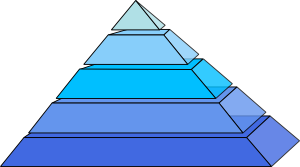
\includegraphics[width=1.1cm]{../Strukturfiler/FIGS/BluePyramid} & \begin{minipage}{\obsl}}{\end{minipage}\\ \end{tabular}\vspace{4mm}\newline}


% = Forudsætning = basis
\newenvironment{basis}{\begin{flushleft} \begin{itshape} }{\end{itshape} \end{flushleft}}


% = Opsummering =
\newenvironment{summary}{\clearpage\pagecolor{sumgul}\section{Opsummering}}{\newpage\pagecolor{white}}











% = Counter
\newcounter{opgavecount}[section]
\setcounter{opgavecount}{0}
\newcounter{spgcount}[opgavecount]
\setcounter{spgcount}{0}
\renewcommand{\thespgcount}{\alph{spgcount})}



% = EXERCISE = (DIVIDER)

\newcommand{\exercisebegin}[1][]{\bigskip\needspace{3\baselineskip}\refstepcounter{opgavecount}\titlegraphic{mingroen}\textcolor{mingroen}{\th{Opgave \theopgavecount \hspace*{1cm} #1}}\medskip\par}

% = QUIZEXERCISE = (DIVIDER)

\newcommand{\quizexercisebegin}[1][]{\bigskip\needspace{3\baselineskip}\refstepcounter{opgavecount}\titlegraphic{mingroen}\textcolor{mingroen}{\th{Quiz-Opgave \theopgavecount \hspace*{1cm} #1}}\medskip\par}

% = QUESTION =

\newenvironment{question}{\refstepcounter{spgcount}\begin{itemize}\item[\thespgcount]}{\end{itemize}\hspace*{\fill}}

% = VINK =

\newenvironment{vink}{\begin{tabular}{m{.9cm}<{\hspace*{2mm}}@{}|m{\obsl}@{}}\hspace*{-4pt}\raggedleft
\includegraphics[width=.9cm]{../Strukturfiler/FIGS/Think} & \begin{minipage}{\obsl}}{\end{minipage}\\ \end{tabular}\medskip\\}
	
% = FACIT =

\newenvironment{facit}{\begin{tabular}{m{.9cm}<{\hspace*{2mm}}@{}|m{\obsl}@{}}\hspace*{-4pt}\raggedleft
\includegraphics[width=.9cm]{../Strukturfiler/FIGS/Check} & \begin{minipage}{\obsl}}{\end{minipage}\\ \end{tabular}\medskip\\}








\newcommand{\afsnit}[1]{\bigskip\th{\titlegraphic{mingroen}\textcolor{mingroen}{#1}} \\ \rule[7pt]{.4\textwidth}{1pt} \vspace*{-2.5mm}\par}

% (DIVIDER):
\newcommand{\ugedagdatotitel}[4]{\pagebreak[4]\section{Semesteruge #1 -- #2 Dag \hspace*{1mm} (#3)} \vspace*{-4mm} \rule[5pt]{\textwidth}{1pt}\vspace*{-2.5mm} \begin{center}\large{\th{#4}}\end{center} \fancyhead[C]{\th{Semesteruge #1}}}

\newenvironment{skema}[1]{\definecolor{shadecolor}{rgb}{0.96,.98, 1.0} \setlength{\FrameSep}{6pt} \renewcommand{\FrameHeightAdjust}{10pt} \vspace*{-4pt}\begin{shaded} \begin{tabular}{#1}}{\end{tabular} \end{shaded} \vspace*{-7pt}}


% ========================

% MAKROER

%\newenvironment{matr}[1][]{\hspace*{-.8mm}\left[\hspace*{-1mm}\begin{array}{#1}}{\end{array}\hspace*{-1mm}\right]\hspace*{-.8mm}}
\newcommand{\bevisslut}{\begin{scriptsize} \begin{flushright} $ \blacksquare $ \end{flushright} \end{scriptsize}}

\newcommand{\tref}[2]{\hyperref[#1]{#2 \ref*{#1}}}
\newcommand{\thref}[2]{\hyperref[#1]{#2}}

\newcommand{\refA}[1]{\colorbox{yellow}{\ref{#1}}}
\newcommand{\hrefA}[2]{\colorbox{yellow}{\href{#1}{#2}}}
\newcommand{\trefA}[2]{\colorbox{yellow}{\hyperref[#1]{#2 \ref*{#1}}}}
\newcommand{\threfA}[2]{\colorbox{yellow}{\hyperref[#1]{#2}}}

\newenvironment{matr}[1]{\hspace*{-.8mm}\begin{bmatrix}\hspace*{-1mm}\begin{array}{#1}}{\end{array}\hspace*{-1mm}\end{bmatrix}\hspace*{-.8mm}}
\newcommand{\transp}{\hspace*{-.6mm}^{\top}}

\newcommand{\maengde}[2]{\left\lbrace \hspace*{-1mm} \begin{array}{c|c} #1 & #2 \end{array} \hspace*{-1mm} \right\rbrace}

\newenvironment{eqnalign}[1]{\setlength{\arraycolsep}{1.3pt}\begin{equation}\begin{array}{#1}}{\end{array}\end{equation}\par}
\newcommand{\eqnl}{\setlength{\arraycolsep}{1.3pt}}

\newcommand{\matind}[3]{{_\mathrm{#1}\mathbf{#2}_\mathrm{#3}}}
\newcommand{\vekind}[2]{{_\mathrm{#1}\mathbf{#2}}}
\newcommand{\jac}[2]{{\mathrm{Jacobi}_\mathbf{#1} (#2)}}
\newcommand{\diver}[2]{{\mathrm{div}\mathbf{#1} (#2)}}
\newcommand{\rot}[1]{{\mathbf{rot}\mathbf{(#1)}}}

\newcommand{\am}{\mathrm{am}}
\newcommand{\gm}{\mathrm{gm}}
\newcommand{\E}{\mathrm{E}}
\newcommand{\Span}{\mathrm{span}}
\newcommand{\mU}{\mathbf{U}}

\newcommand{\ms}{\medskip\\}
\newcommand{\bs}{\bigskip\\}

\newcommand{\mA}{\mathbf{A}}
\newcommand{\mB}{\mathbf{B}}
\newcommand{\mC}{\mathbf{C}}
\newcommand{\mD}{\mathbf{D}}
\newcommand{\mE}{\mathbf{E}}
\newcommand{\mF}{\mathbf{F}}
\newcommand{\mK}{\mathbf{K}}
\newcommand{\mI}{\mathbf{I}}
\newcommand{\mM}{\mathbf{M}}
\newcommand{\mN}{\mathbf{N}}
\newcommand{\mQ}{\mathbf{Q}}
\newcommand{\mT}{\mathbf{T}}
\newcommand{\mV}{\mathbf{V}}
\newcommand{\mW}{\mathbf{W}}
\newcommand{\mX}{\mathbf{X}}
\newcommand{\ma}{\mathbf{a}}
\newcommand{\mb}{\mathbf{b}}
\newcommand{\mc}{\mathbf{c}}
\newcommand{\md}{\mathbf{d}}
\newcommand{\me}{\mathbf{e}}
\newcommand{\mn}{\mathbf{n}}
\newcommand{\mr}{\mathbf{r}}
\newcommand{\mv}{\mathbf{v}}
\newcommand{\mw}{\mathbf{w}}
\newcommand{\mx}{\mathbf{x}}
\newcommand{\mxb}{\mathbf{x_{bet}}}
\newcommand{\my}{\mathbf{y}}
\newcommand{\mz}{\mathbf{z}}
\newcommand{\reel}{\mathbb{R}}
\newcommand{\mL}{\bm{\Lambda}} %Lambda-matrix
\newcommand{\mnul}{\bm{0}}
\newcommand{\trap}[1]{\mathrm{trap}(#1)}
\newcommand{\Det}{\operatorname{Det}}
\newcommand{\adj}{\operatorname{adj}}
\newcommand{\Ar}{\operatorname{Areal}}
\newcommand{\Vol}{\operatorname{Vol}}
\newcommand{\Rum}{\operatorname{Rum}}
\newcommand{\diag}{\operatorname{\bf{diag}}}
\newcommand{\bidiag}{\operatorname{\bf{bidiag}}}
\newcommand{\spanVec}[1]{\mathrm{span}\{#1\}}
\newcommand{\Div}{\operatorname{Div}}
\newcommand{\Rot}{\operatorname{\mathbf{Rot}}}

\newcommand{\Jac}{\operatorname{Jacobi}}
\newcommand{\Tan}{\operatorname{Tan}}
\newcommand{\Ort}{\operatorname{Ort}}
\newcommand{\Flux}{\operatorname{Flux}}
\newcommand{\Cmass}{\operatorname{Cm}}
\newcommand{\Imom}{\operatorname{Im}}
\newcommand{\Pmom}{\operatorname{Pm}}
\newcommand{\IS}{\operatorname{I}}
\newcommand{\IIS}{\operatorname{II}}
\newcommand{\IIIS}{\operatorname{III}}
\newcommand{\Le}{\operatorname{L}}
\newcommand{\app}{\operatorname{app}}
\newcommand{\M}{\operatorname{M}}
\newcommand{\re}{\mathrm{Re}}
\newcommand{\im}{\mathrm{Im}}

\newcommand{\compl}{\mathbb{C}} %de komplekse tal
\newcommand{\e}{\mathrm{e}} %eksponentialfunktionen. lodret 'e', og altså ikke kursiv ligesom andre bogstaver.





% Medialink: SCREEN: (QRcode) + thumbnail image + link på kodenummer (til qr.dtu.dk)
\newcommand{\onlinemedia}[3]{
	\begin{wrapfigure}{r}{3.2cm} 
		\vspace{-30pt} 
		\vspace{#1pt} 
		\begin{flushright} 
			\includegraphics[width=3cm]{qr/#2.png} 
			\tiny 
			\href{http://qr.dtu.dk/#2}{#2: #3}
			\normalsize  
		\end{flushright} 
		\vspace{-10pt} 
	\end{wrapfigure}
}
\newcommand{\onlinemediathumb}[3]{
	\begin{wrapfigure}{r}{3.2cm} 
		\vspace{-30pt} 
		\vspace{#1pt} 
		\begin{flushright} 
			\includegraphics[width=3cm]{qr/#2.png} 
			\includegraphics[width=3cm]{qr/#2_thumb.png} 
			\tiny 
			\href{http://qr.dtu.dk/#2}{#2: #3}
			\normalsize  
		\end{flushright} 
		\vspace{-10pt} 
	\end{wrapfigure}
}



% Index:
\usepackage{makeidx}
\makeindex
\newcommand\ind[2]{\index{#1}\textbf{\textit{\textcolor{black}{#2}}}}

% ###SERVER_EXCLUDE_BEGIN###
\externaldocument[NUID17-]{../../enoten/TN01-Talrum/Talrum}
\externaldocument[NUID1-]{../../enoten/TN02-Ligningssystemer/TNdriver}
\externaldocument[NUID2-]{../../enoten/TN03-Matricer_og_Matrixalgebra/Matricer_og_matrixalgebra}
\externaldocument[NUID3-]{../../enoten/TN04-Kvadratiske_matricer/TNdriver}
\externaldocument[NUID11-]{../../enoten/TN05-Determinanter/Determinanter}
\externaldocument[NUID12-]{../../enoten/TN06-GeometriskeVektorer/GeometriskeVektorer}
\externaldocument[NUID18-]{../../enoten/TN07-Vektorrum/VektorRum}
\externaldocument[NUID21-]{../../enoten/TN08-LinAfbildninger/LinAfbildninger}
\externaldocument[NUID23-]{../../enoten/TN09-Egenvaerdier_og_egenvektorer/TNdriver}
\externaldocument[NUID24-]{../../enoten/TN10-Diagonalisering_med_egenvektorer/TNdriver}
\externaldocument[NUID10-]{../../enoten/TN11-1.ordens_differentialligninger/TNdriver}
\externaldocument[NUID13-]{../../enoten/TN12-1.ordens_differentialligningssystemer/TNdriver}
\externaldocument[NUID14-]{../../enoten/TN13-2.ordens_differentialligninger/TNdriver}
\externaldocument[NUID27-]{../../enoten/TN14-Elemenataere_funktioner/Elementaere_Funktioner}
\externaldocument[NUID28-]{../../enoten/TN15-Funktioner2Variable/Funktioner_To_Variable}
\externaldocument[NUID29-]{../../enoten/TN16-Gradienter_og_Tangentplaner/Gradienter_og_Tangentplaner}
\externaldocument[NUID32-]{../../enoten/TN17-Taylor_formler/Taylor_Formler}
\externaldocument[NUID33-]{../../enoten/TN18-Taylor_2Var/Taylor_2Var}
\externaldocument[NUID34-]{../../enoten/TN19-SymMat/SymmetriskeMatricer}
\externaldocument[NUID35-]{../../enoten/TN20-KegleSnit/Keglesnit}
\externaldocument[NUID36-]{../../enoten/TN21-Riemann_Integral/Riemann_01}
\externaldocument[NUID37-]{../../enoten/TN22-Plan_Int/Plan_Int_01}
\externaldocument[NUID39-]{../../enoten/TN23-Flade_Int/Flade_Rum_Int_01}
\externaldocument[NUID40-]{../../enoten/TN24-Vektorfelter/Vektorfelter_01}
\externaldocument[NUID41-]{../../enoten/TN25-Flux/Flux_02}
\externaldocument[NUID42-]{../../enoten/TN26-Gauss/Gauss_01}
\externaldocument[NUID128-]{../../enoten/TN27-Stokes/Stokes_01}
\externaldocument[NUID43-]{../../enoten/TN29-KomplekseTal/KomplekseTal}

\externaldocument[NUID6-]{../../E-math-opgaver/Opgaver/opgU123}
\externaldocument[NUID19-]{../../E-math-opgaver/Opgaver/opgU45}
\externaldocument[NUID20-]{../../E-math-opgaver/Opgaver/opgU678}
\externaldocument[NUID25-]{../../E-math-opgaver/Opgaver/opgU910SD}
\externaldocument[NUID31-]{../../E-math-opgaver/OpgaverF11-U123/opgF123}
% \externaldocument[NUID9-]{../../E-math-opgaver/Opgaver/Dagsordner E10}
% ###SERVER_EXCLUDE_END###


% Begin document and set alternative chapter title:
\begin{document}
\renewcommand{\chaptername}{eNote}

\setcounter{chapter}{20} %SÆT DETTE TAL TIL 1 MINDRE END DET AKTUELLE TRANSFERNOTE-NUMMER!!

%%%%%%%%%%%%%%%%%%%%%%%%%%%%%%%%%%%%%%%%%%%%%
%%%%%%%%%%%%%%%%%%%%%%%%%%%%%%%%%%%%%%%%%%%%%
%%% HERFRA SKAL DU SKRIVE ELLER INDSÆTTE %%%%
%%% DEN FIL DU ØNSKER %%%%%%%%%%%%%%%%%%%%%%%
%%%%%%%%%%%%%%%%%%%%%%%%%%%%%%%%%%%%%%%%%%%%%
%%%%%%%%%%%%%%%%%%%%%%%%%%%%%%%%%%%%%%%%%%%%%


% REF: TransferNote \ref{TN4-tn4} \nameref{TN4-tn4}
%
% \tref{NUID14-thm.koma}{sætning} \tref{NUID28-tn15}{eNote}
%
%\tref{NUID34-tn19}{eNote} Symmetriske matricer
%\tref{NUID33-tn18}{eNote} Taylor i 2 variable
%
% 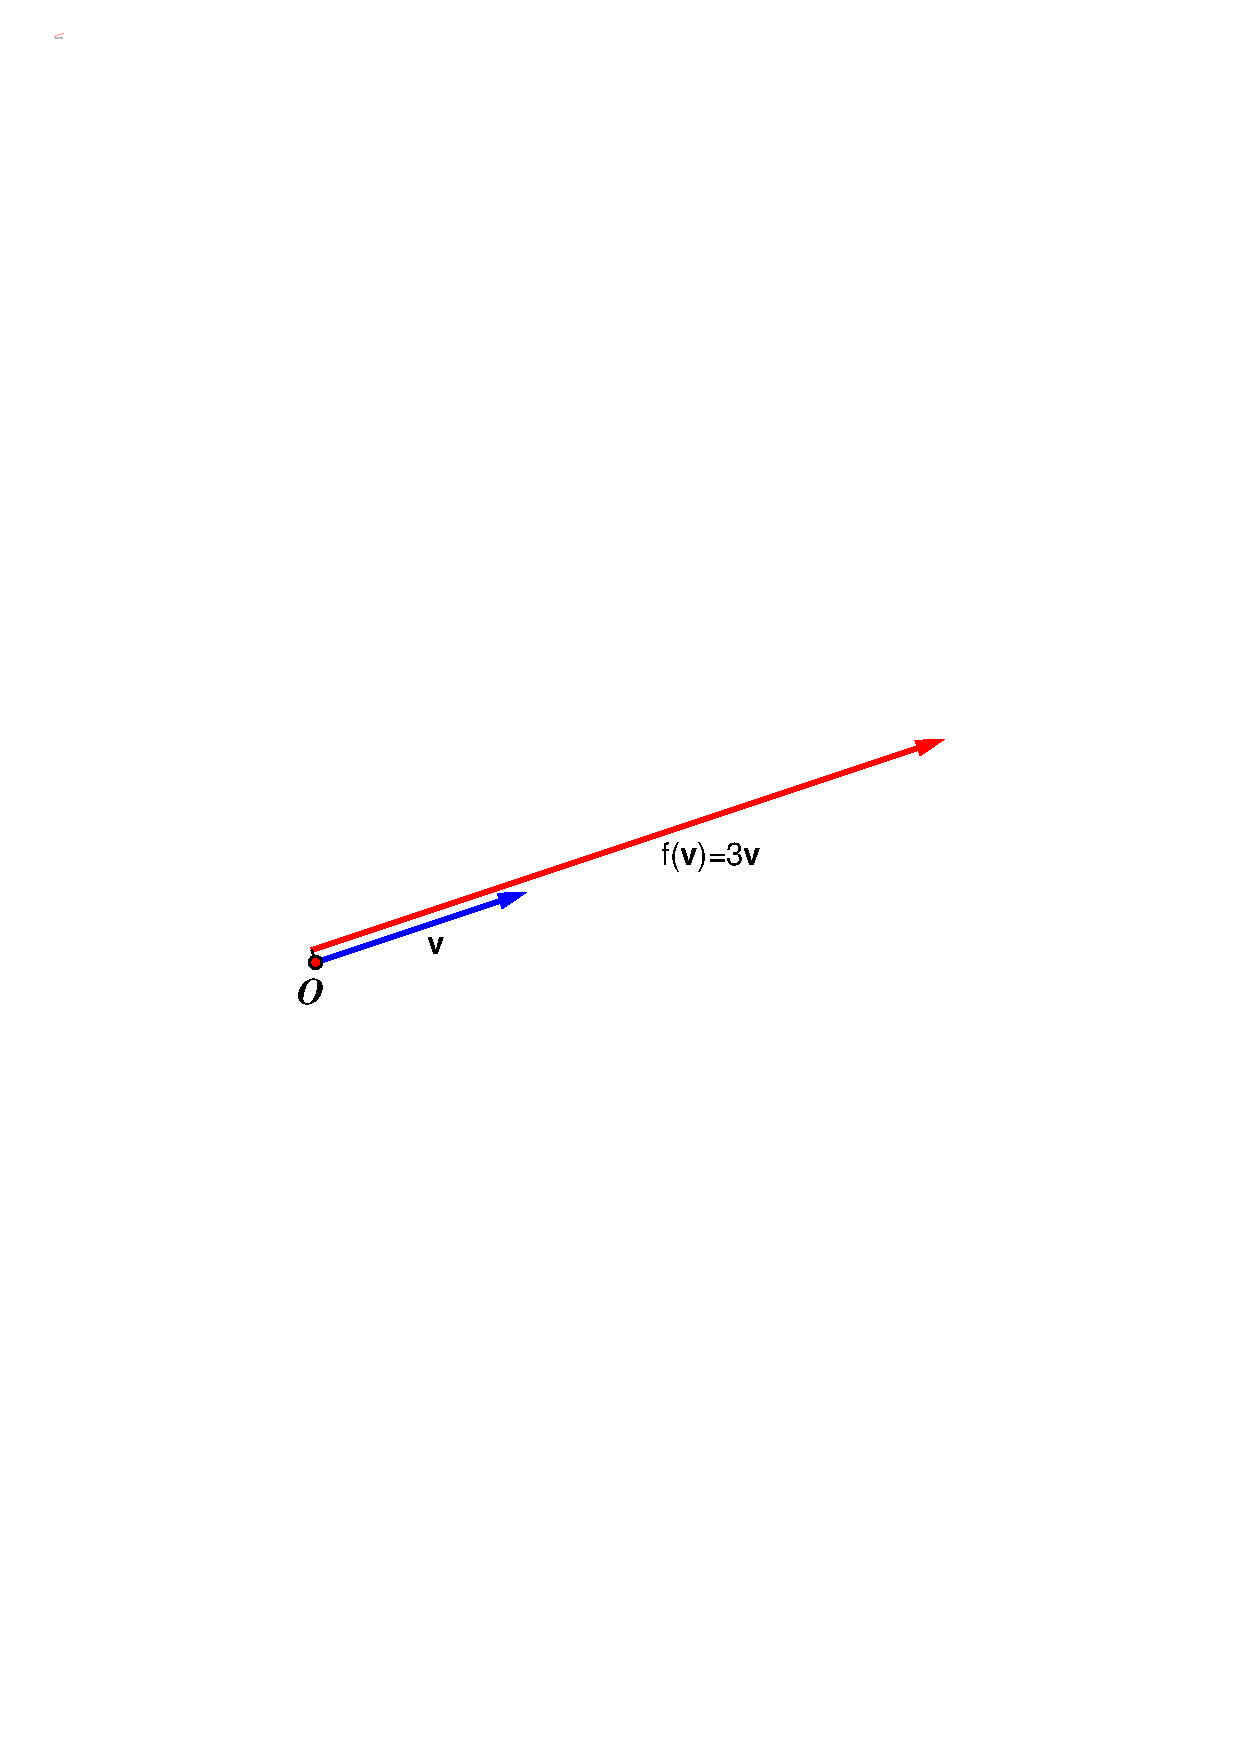
\includegraphics[trim=5cm 12cm 5cm 12cm,width=0.40\textwidth,clip]{skalering.pdf}
%
%\begin{equation}
%\matind vMa \cdot \matind aFa \cdot \matind aMv = \matind vFv \, ,
%\end{equation}
%hvor
%\begin{equation}
%\matind aMv = \begin{matr}{cccc} \vekind av_1 & \vekind av_2 & \cdots & \vekind av_n \end{matr} \quad \mathrm{og} \quad %\matind vFv = \diag(\lambda_1, \lambda_2, \ldots, \lambda_n) \, .
%\end{equation}
%
%$\vekind{e}{F}$
%$\matind{e}{F}{w}$
%%%%%%%%%%%%%%%%%%%%%%%%%%%%%%%%%%%%%%%%%%%%%%%%%%%
%%%%%%%%%%%%%%%%%%%%%%%%%%%%%%%%%%%%%%%%%%%%%%%%%%%
%%%%%%%%%%%%%%%%%%%%%%%%%%%%%%%%%%%%%%%%%%%%%%%%%%%
%%%%%%%%%%%%%%%%%%%%%%%%%%%%%%%%%%%%%%%%%%%%%%%%%%%



\chapter{Riemann-integraler} \label{tn21}

\begin{basis}
I denne eNote vil vi opstille og give eksempler på de teknikker, metoder, og resultater, som er helt nødvendige hjælpemidler når vi skal finde
længder af kurver, arealer af plane områder og af overflader, samt rumfang, massemidtpunkter, og inertimomenter af rumlige områder etc. Det handler i første omgang om at kunne integrere og om at kunne finde stamfunktioner
til givne kontinuerte funktioner, især til funktioner af \'{e}n variabel. Vi vil derfor et par gange referere til \tref{NUID27-tn14}{eNote}. Vi skal i denne eNote se hvordan uendelige summer af uendeligt små addender i grænsen fører til de såkaldte Riemann-integraler, som igen kan udtrykkes og beregnes ved brug af passende stamfunktioner. Metoderne og de fundamentale resultater for Riemann-integralerne er ikke afgørende forskellige i de dimensioner vi betragter,
men vi vil alligevel diskutere og analysere betegnelser, resultater, og eksempler helt eksplicit for funktioner af \'{e}n, to, og tre variable med henblik på at kunne bruge Riemann-integralerne mest effektivt i de anvendelser, som dyrkes i de eNoter der handler om integration i flere variable.
\end{basis}



%%%%%%%%%%%%%%%%%%%%%%%%%%%%%%%%%%%%%%%%%%%%%%%%%%%%%%%%%%%%%
%%%%%%%%%%%%%%%%%%%%%%%%%%%%%%%%%%%%%%%%%%%%%%%%%%%%%%%%%%%%%
%%%%%%%%%%%%%%%%%%%%%%%%%%%%%%%%%%%%%%%%%%%%%%%%%%%%%%%%%%%%%












%%%%%%%%%%%%%%%%%%%%%%%%%%%%%%%%%%%%%%%%%%%%%%%%%%%%%%%%%%%%%%%%%%%%%%%%%%%%
%%%%%%%%%%%%%%%%%%%%%%%%%%%%%%%%%%%%%%%%%%%%%%%%%%%%%%%%%%%%%%%%%%%%%%%%%%%%
\section{Indledning} \label{secIndledning}

Ideen med denne og de efterfølgende eNoter er at motivere, opstille, og anvende det unikke
værktøj, der kan besvare spørgsmål som helt naturligt opstår i mangfoldige sammenhænge: Hvor lang
er den kurve? Hvor stort er det område i planen?
Hvad vejer det fladestykke? Hvad er rumfanget af
det område i rummet? Hvad er energi-optaget på
det solfangertag i løbet af i dag? Hvor meget
deformeres det legeme, når det flyder langs det
vektorfelt?\\

Det værktøj -- den metode -- der kan besvare disse
spørgsmål, hedder {\emph{integration}}. Det vil sige, vi skal kunne integrere givne funktioner $f(x)$ og finde stamfunktioner til dem. Som bekendt er en stamfunktion til $f(x)$ en funktion $F(x)$ hvis differentialkvotient er $f(x)$. Men dem er der jo mange af; hvis vi differentierer $F(x) + c$, hvor $c$ er en konstant, så får vi igen $f(x)$. Det vil sige, hvis $F(x)$ er en stamfunktion, så er $F(x) + c$ også en stamfunktion!\\


Derudover er det på ingen måde på forhånd klart, at sådanne stamfunktioner skulle have noget som helst at gøre med
længder, arealer, rumfang, eller vægt. Og hvilken funktion $f(x)$ skal vi iøvrigt bruge,
når vi  for eksempel vil finde rumfanget af en kugle? Og hvis vi ellers kan finde en stamfunktion
til $f(x)$, hvilken konstant skal der så lægges til for at vi kan få det rigtige rumfang? For at få en ide om det, må vi først se på, hvordan vi i det hele taget kan prøve på at {\emph{definere}} hvad vi skal forstå ved begrebet rumfang.


\begin{figure}[ht]
\centerline{  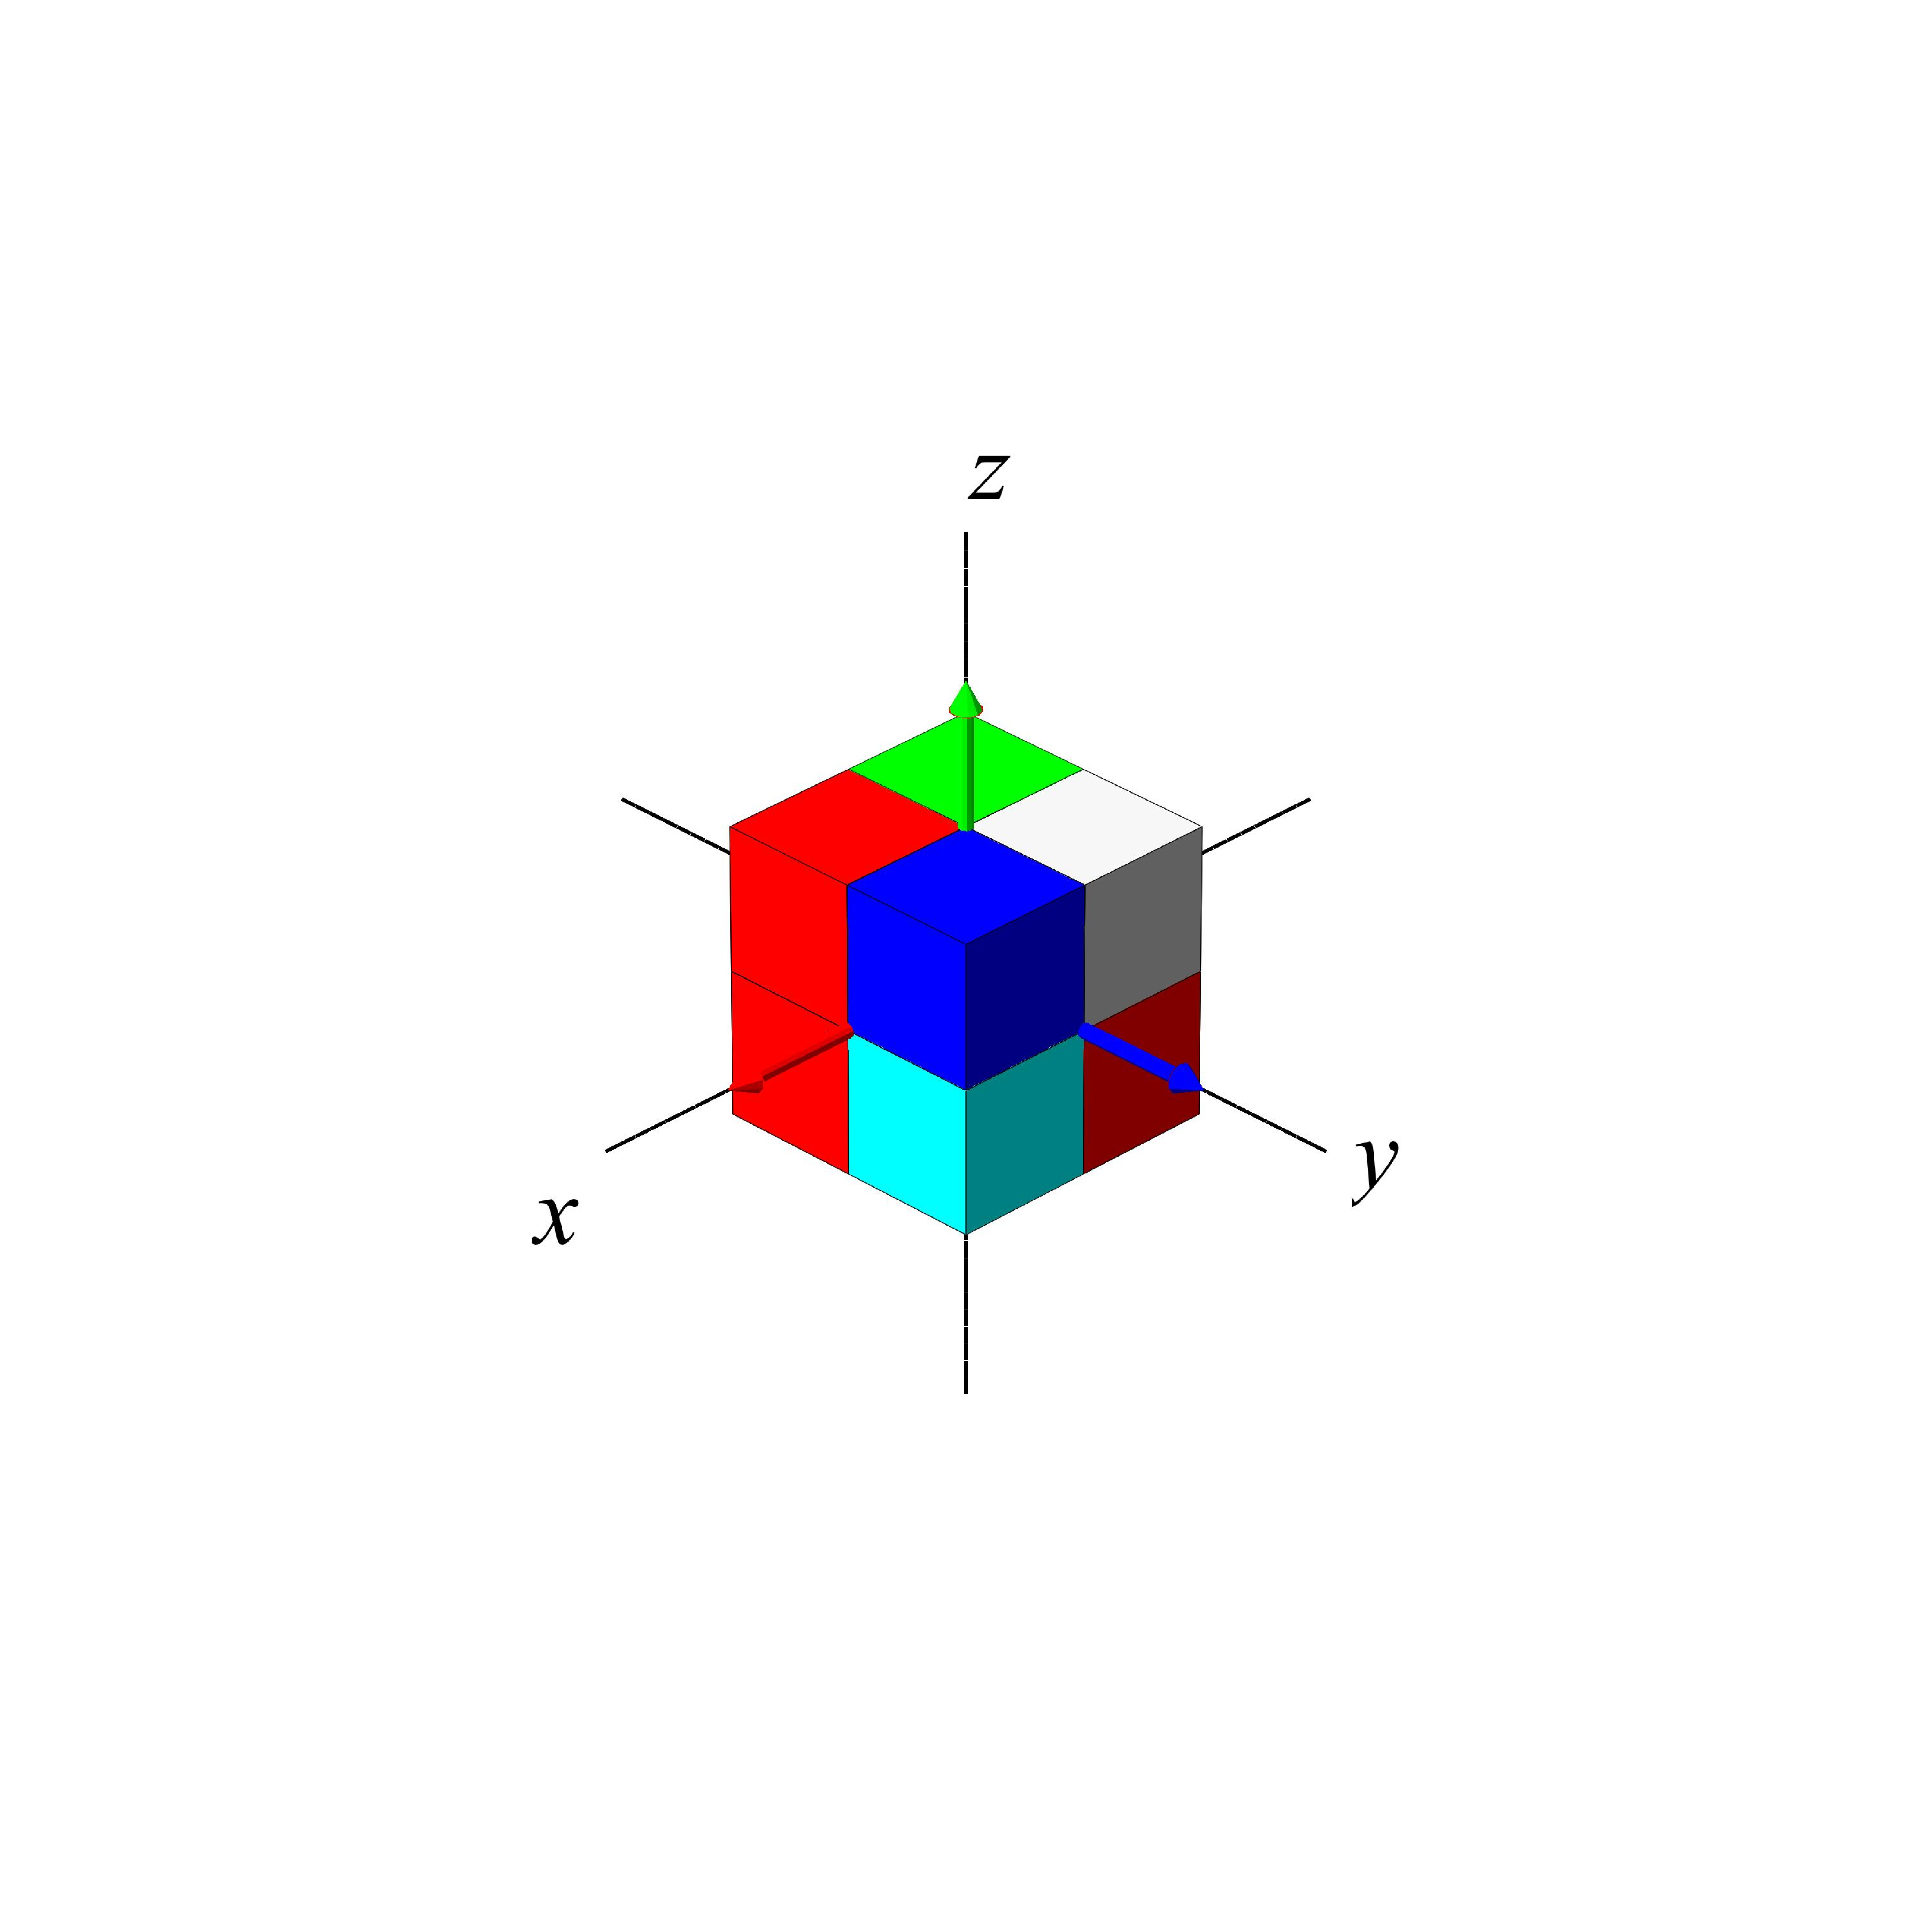
\includegraphics[height=60mm]{FIGS/plotSphereFillB.pdf}  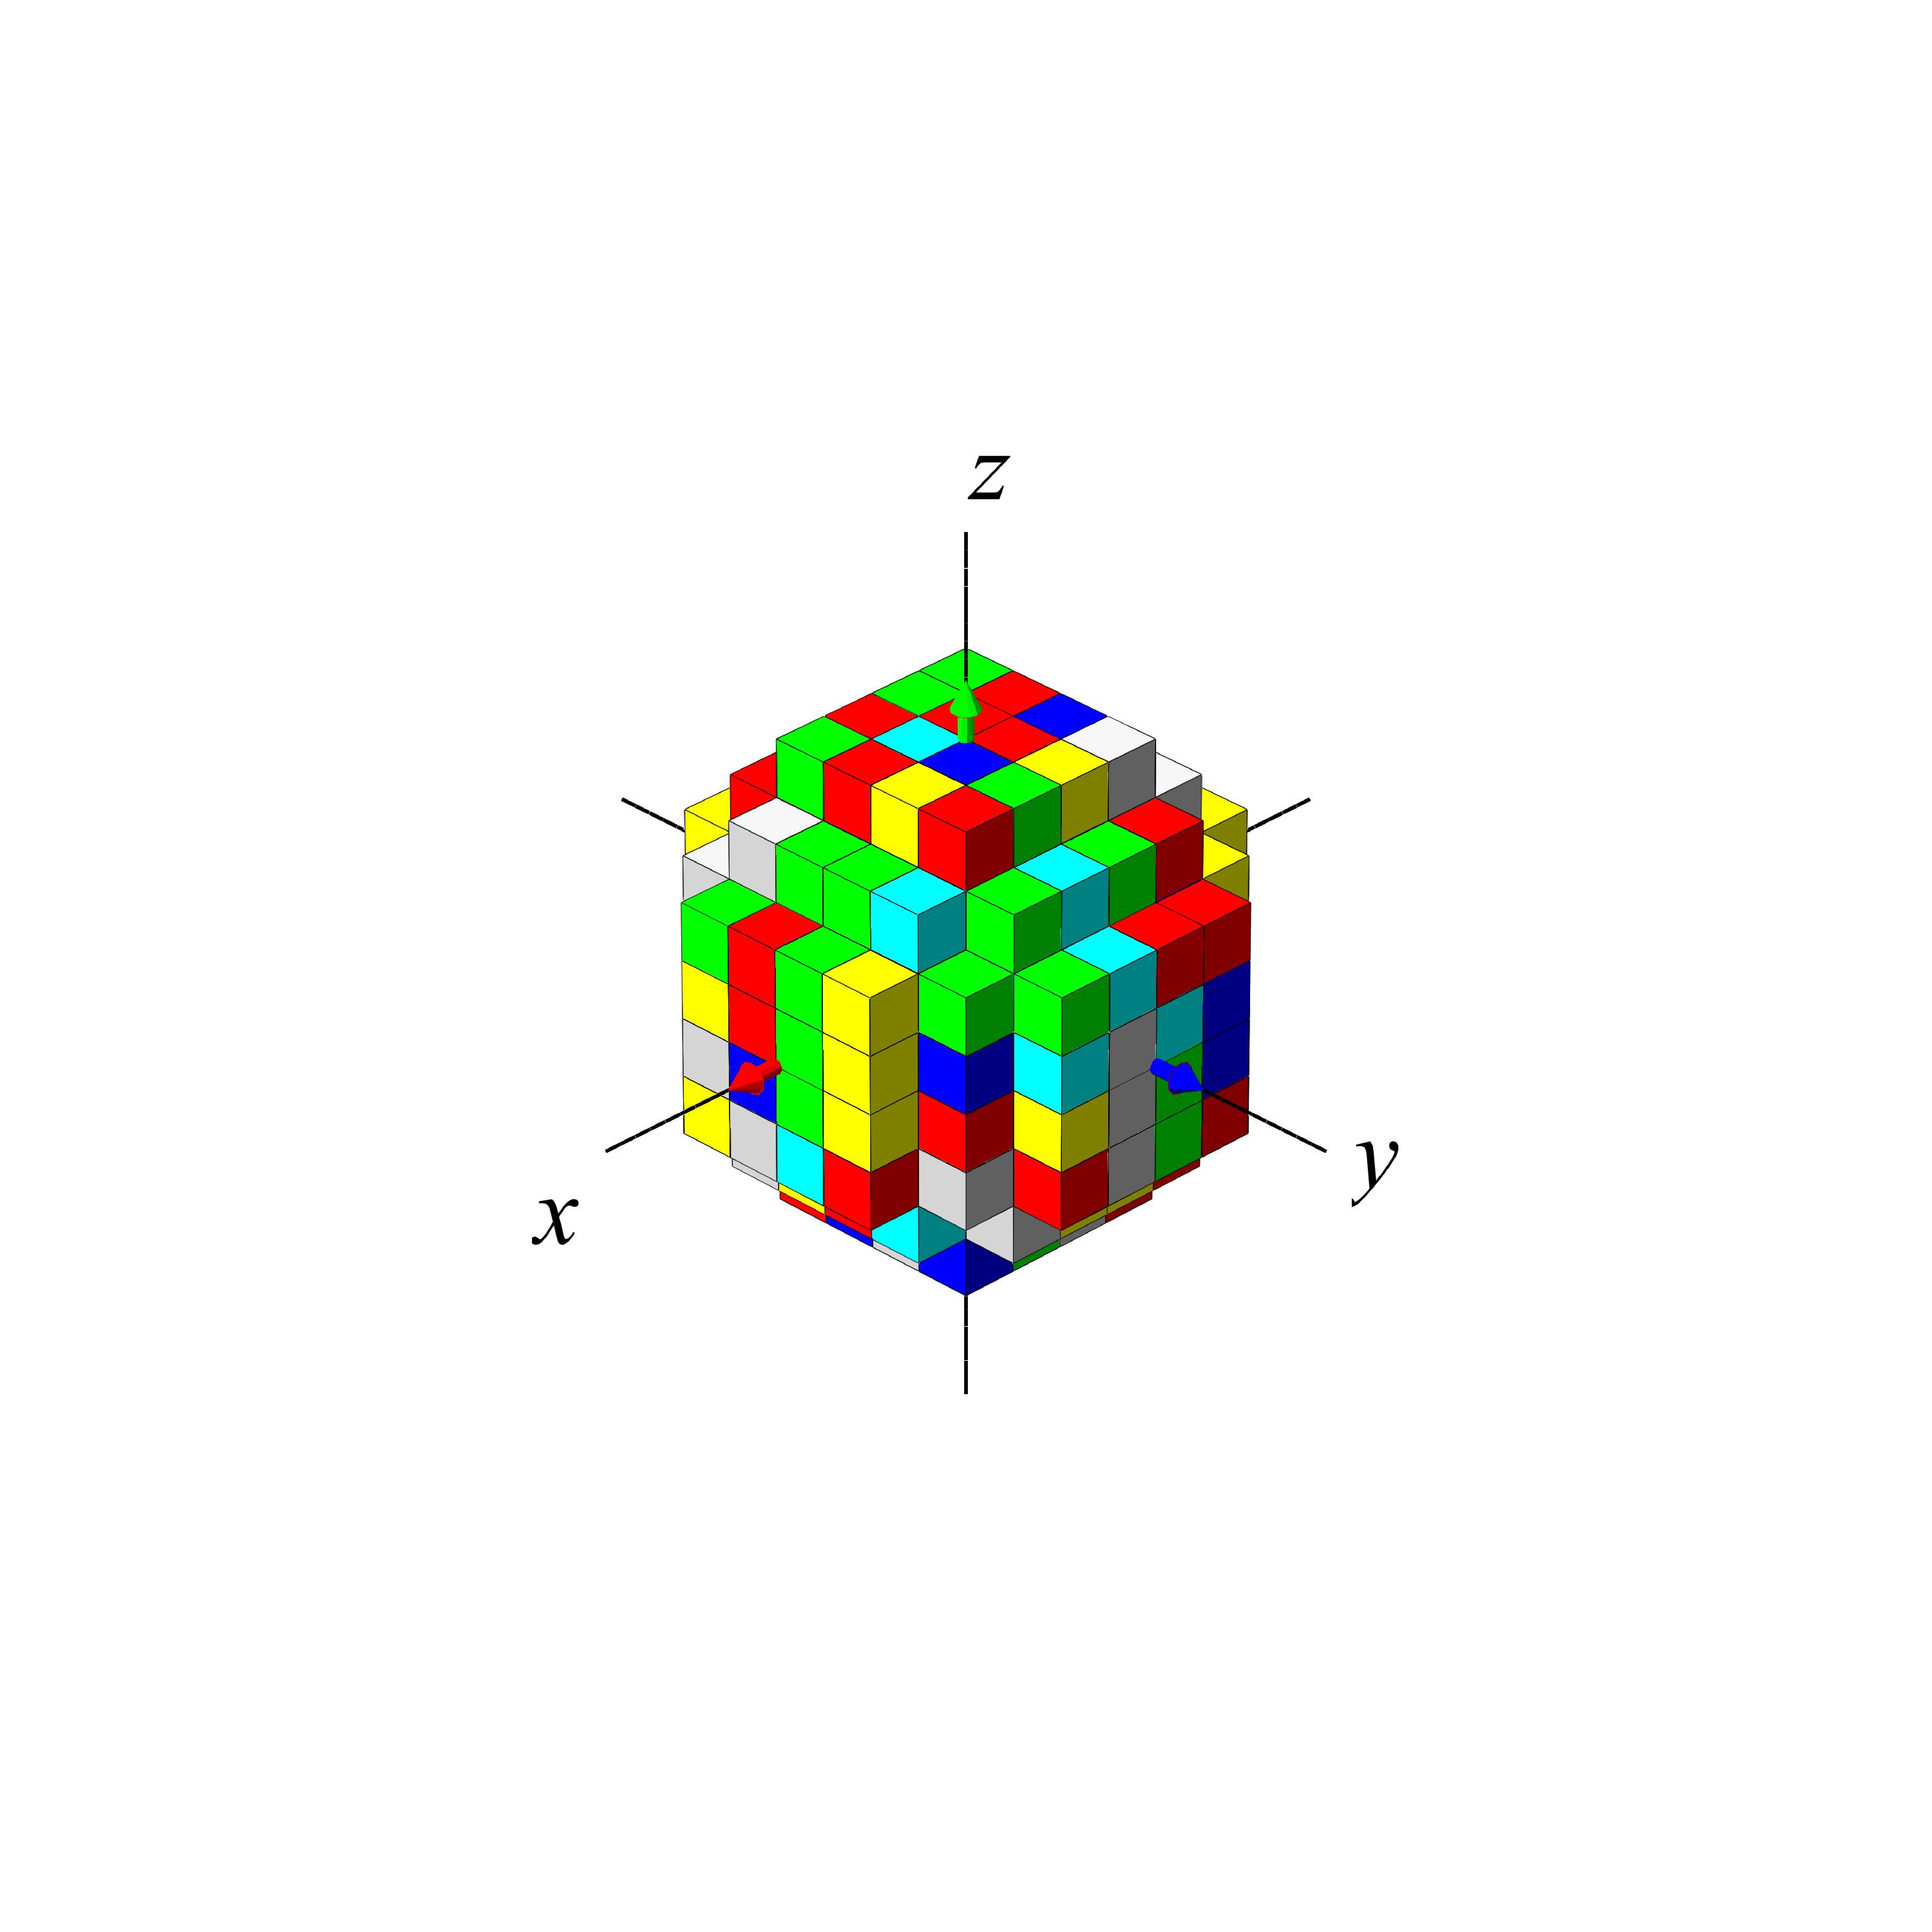
\includegraphics[height=60mm]{FIGS/plotSphereFillC.pdf}  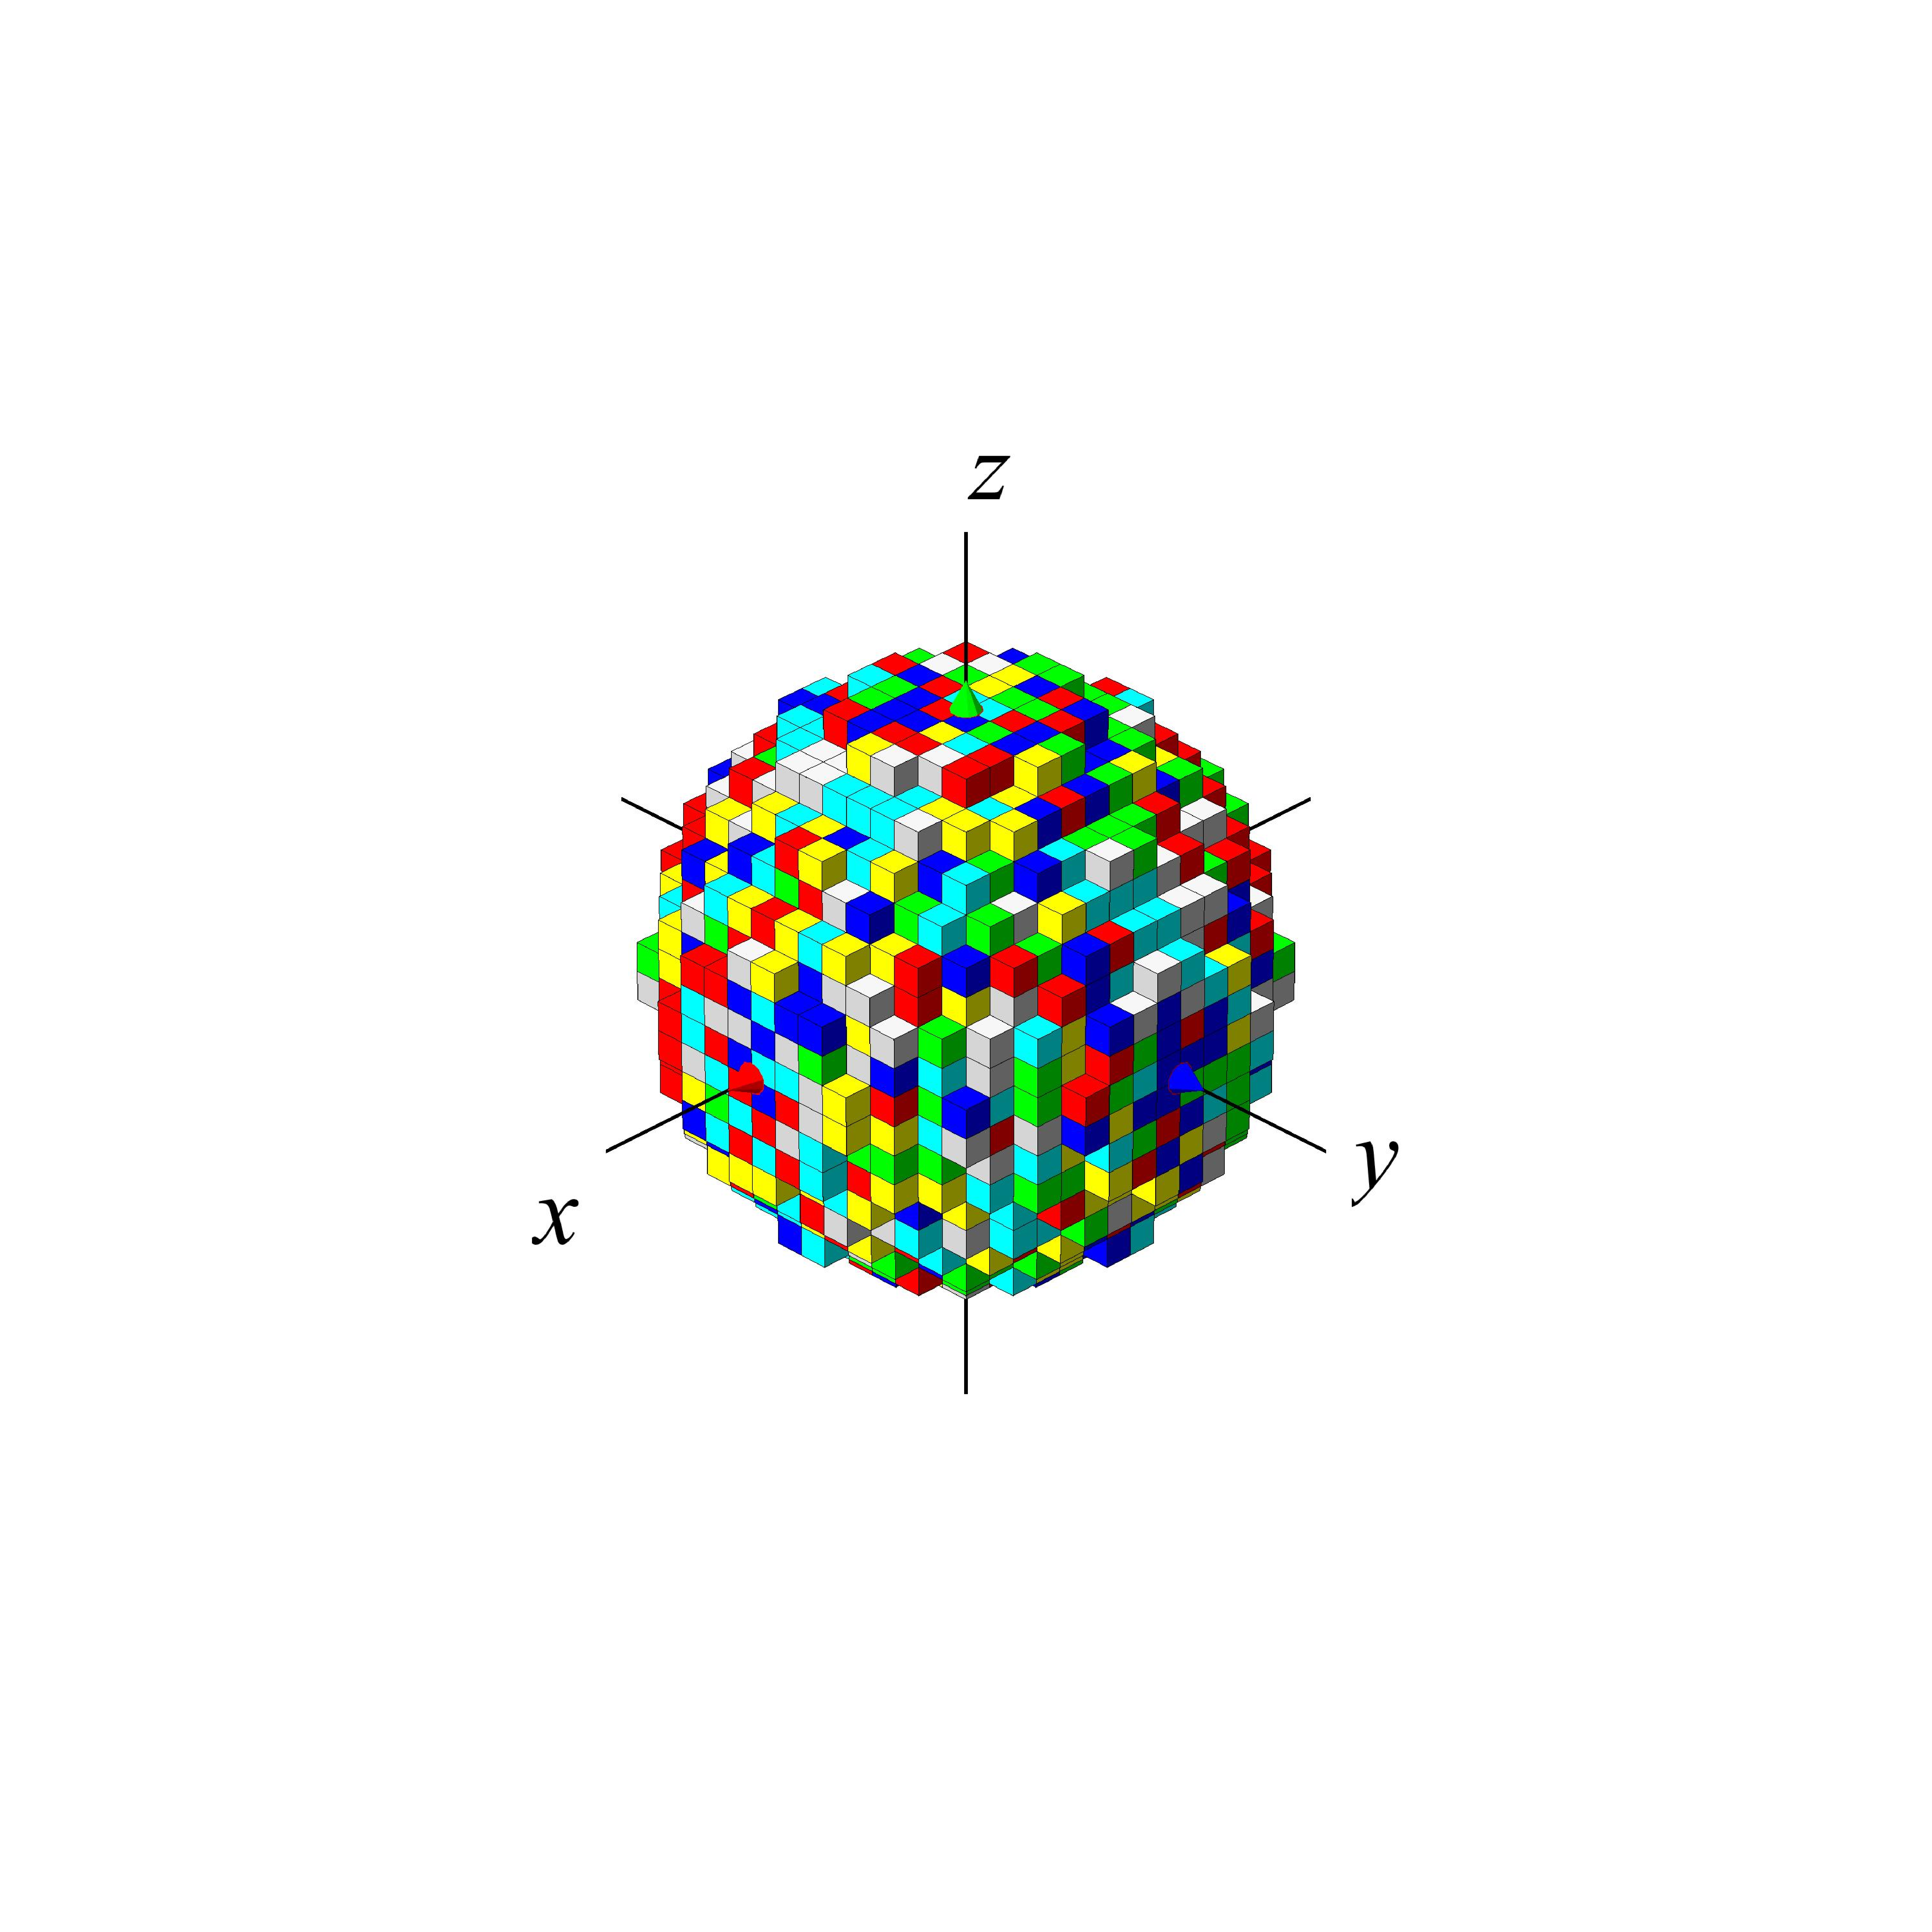
\includegraphics[height=60mm]{FIGS/plotSphereFillD.pdf}}
\begin{center}
\caption{\small{Kuglefyldninger med kubiske klodser. Den antydede kugle, som ønskes fyldt med klodserne, har radius $1$.
Til venstre er der plads i kuglen til $8$ klodser hver med sidelængde $0.5$; i midten er der brugt 304 klodser, hver med sidelængden $0.2$; til højre er
benyttet 3280 klodser, hver med sidelængden $0.1$.}}
\label{figSphereFill}
\end{center}
\end{figure}




\section{Rumfang-problemet} \label{secRumfang}
Rumfanget af et givet område i rummet, f.eks. en massiv
kugle med radius $1$,  kan bygges op af
standard-elementer med simplest mulig kasseformet
geometri, for eksempel kubiske klodser. Men resultatet af en sådan opbygning af kuglen kan jo kun
blive en grov tilnærmelse til kuglen, se figur \ref{figSphereFill}. Og summen af de kubiske
klodsers rumfang er derfor kun en grov tilnærmelse til
kuglens rumfang. \\

Hvis vi imidlertid fylder den samme kugle med kubiske
klod\-ser, der hver for sig har 1000 gange
mindre rumfang (altså 10 gange mindre sidelængde) er det klart, at den ønskede
kugle derved kan tilnærmes meget bedre ved brug af (mere end 1000 gange) flere
kubiske klodser; og det
er stadig (i princippet) en simpel sag at lægge
alle klodsernes rumfang sammen. Det giver dermed
også en meget bedre værdi for rumfanget af
kuglen. \\

\begin{aha}
Eksemplet i Figur \ref{figSphereFill} viser princippet:
Approksimationen af en kugle med radius $1$ med $8$ kubiske klodser med sidelængde $1/2$ har rumfanget $8\cdot (1/2)^{3} = 1$; i midten har vi  $304$ kubiske klodser (alle med sidelængde $1/5$) der giver et
tilnærmet rumfang på $304\cdot (1/5)^{3} \, = \, 2.432$, mens approksimationen
med $3280$ klodser (med sidelængde $0.1$) i højre figur klart giver en endnu bedre tilnærmelse:
$3280\cdot (1/10)^{3} \, = \, 3.280$. Til sammenligning vidste allerede Archimedes,
at det eksakte volumen af enhedskuglen er $4\pi/3 \, \approx \, 4.1888\,.$\\
\end{aha}


Når først dette er klart, så er ønsket
selvfølgelig at 'gå til grænsen' ved at lade antallet
af standard-klodser gå imod uendelig samtidig med
at de benyttede klodser gøres tilsvarende mindre i
hvert forsøg. Og således pakke og udfylde kuglen bedre og bedre, med flere og flere, mindre og mindre kuber, og derved opnå \ind{Archimedes' resultat}{Archimedes' resultat} i grænsen. \\

Men
hvordan lægger vi uendelig mange uendelig små
rumfang sammen? Og går det virkelig godt?
Integrationsbegrebet og de tilhørende stamfunktionsbestemmelser giver præcise anvisninger og
overraskende positive svar på begge disse
spørgsmål. \\

Vi viser i denne eNote
hvilke formelle overvejelser og metoder, der ligger bag den
succes og tager dernæst straks i de efterfølgende eNoter fat på at bruge integrationsteknikkerne
til at bestemme længder af kurver, arealer af fladestykker, rumfang af
rumlige områder,
etc.\\


I eNoten om integration i tre variable vises for eksempel, hvordan kuglens rumfang kan beregnes eksakt ved hjælp af 'udfyldninger' med
kasseformede blokke (med forskellig størrelse og form i stil med udfyldningerne af kuglen ovenfor), se figurerne \ref{figSphereFill},
\ref{figKugleskal} og eksempel \ref{exampKugle}.


\begin{figure}[h]
\centerline{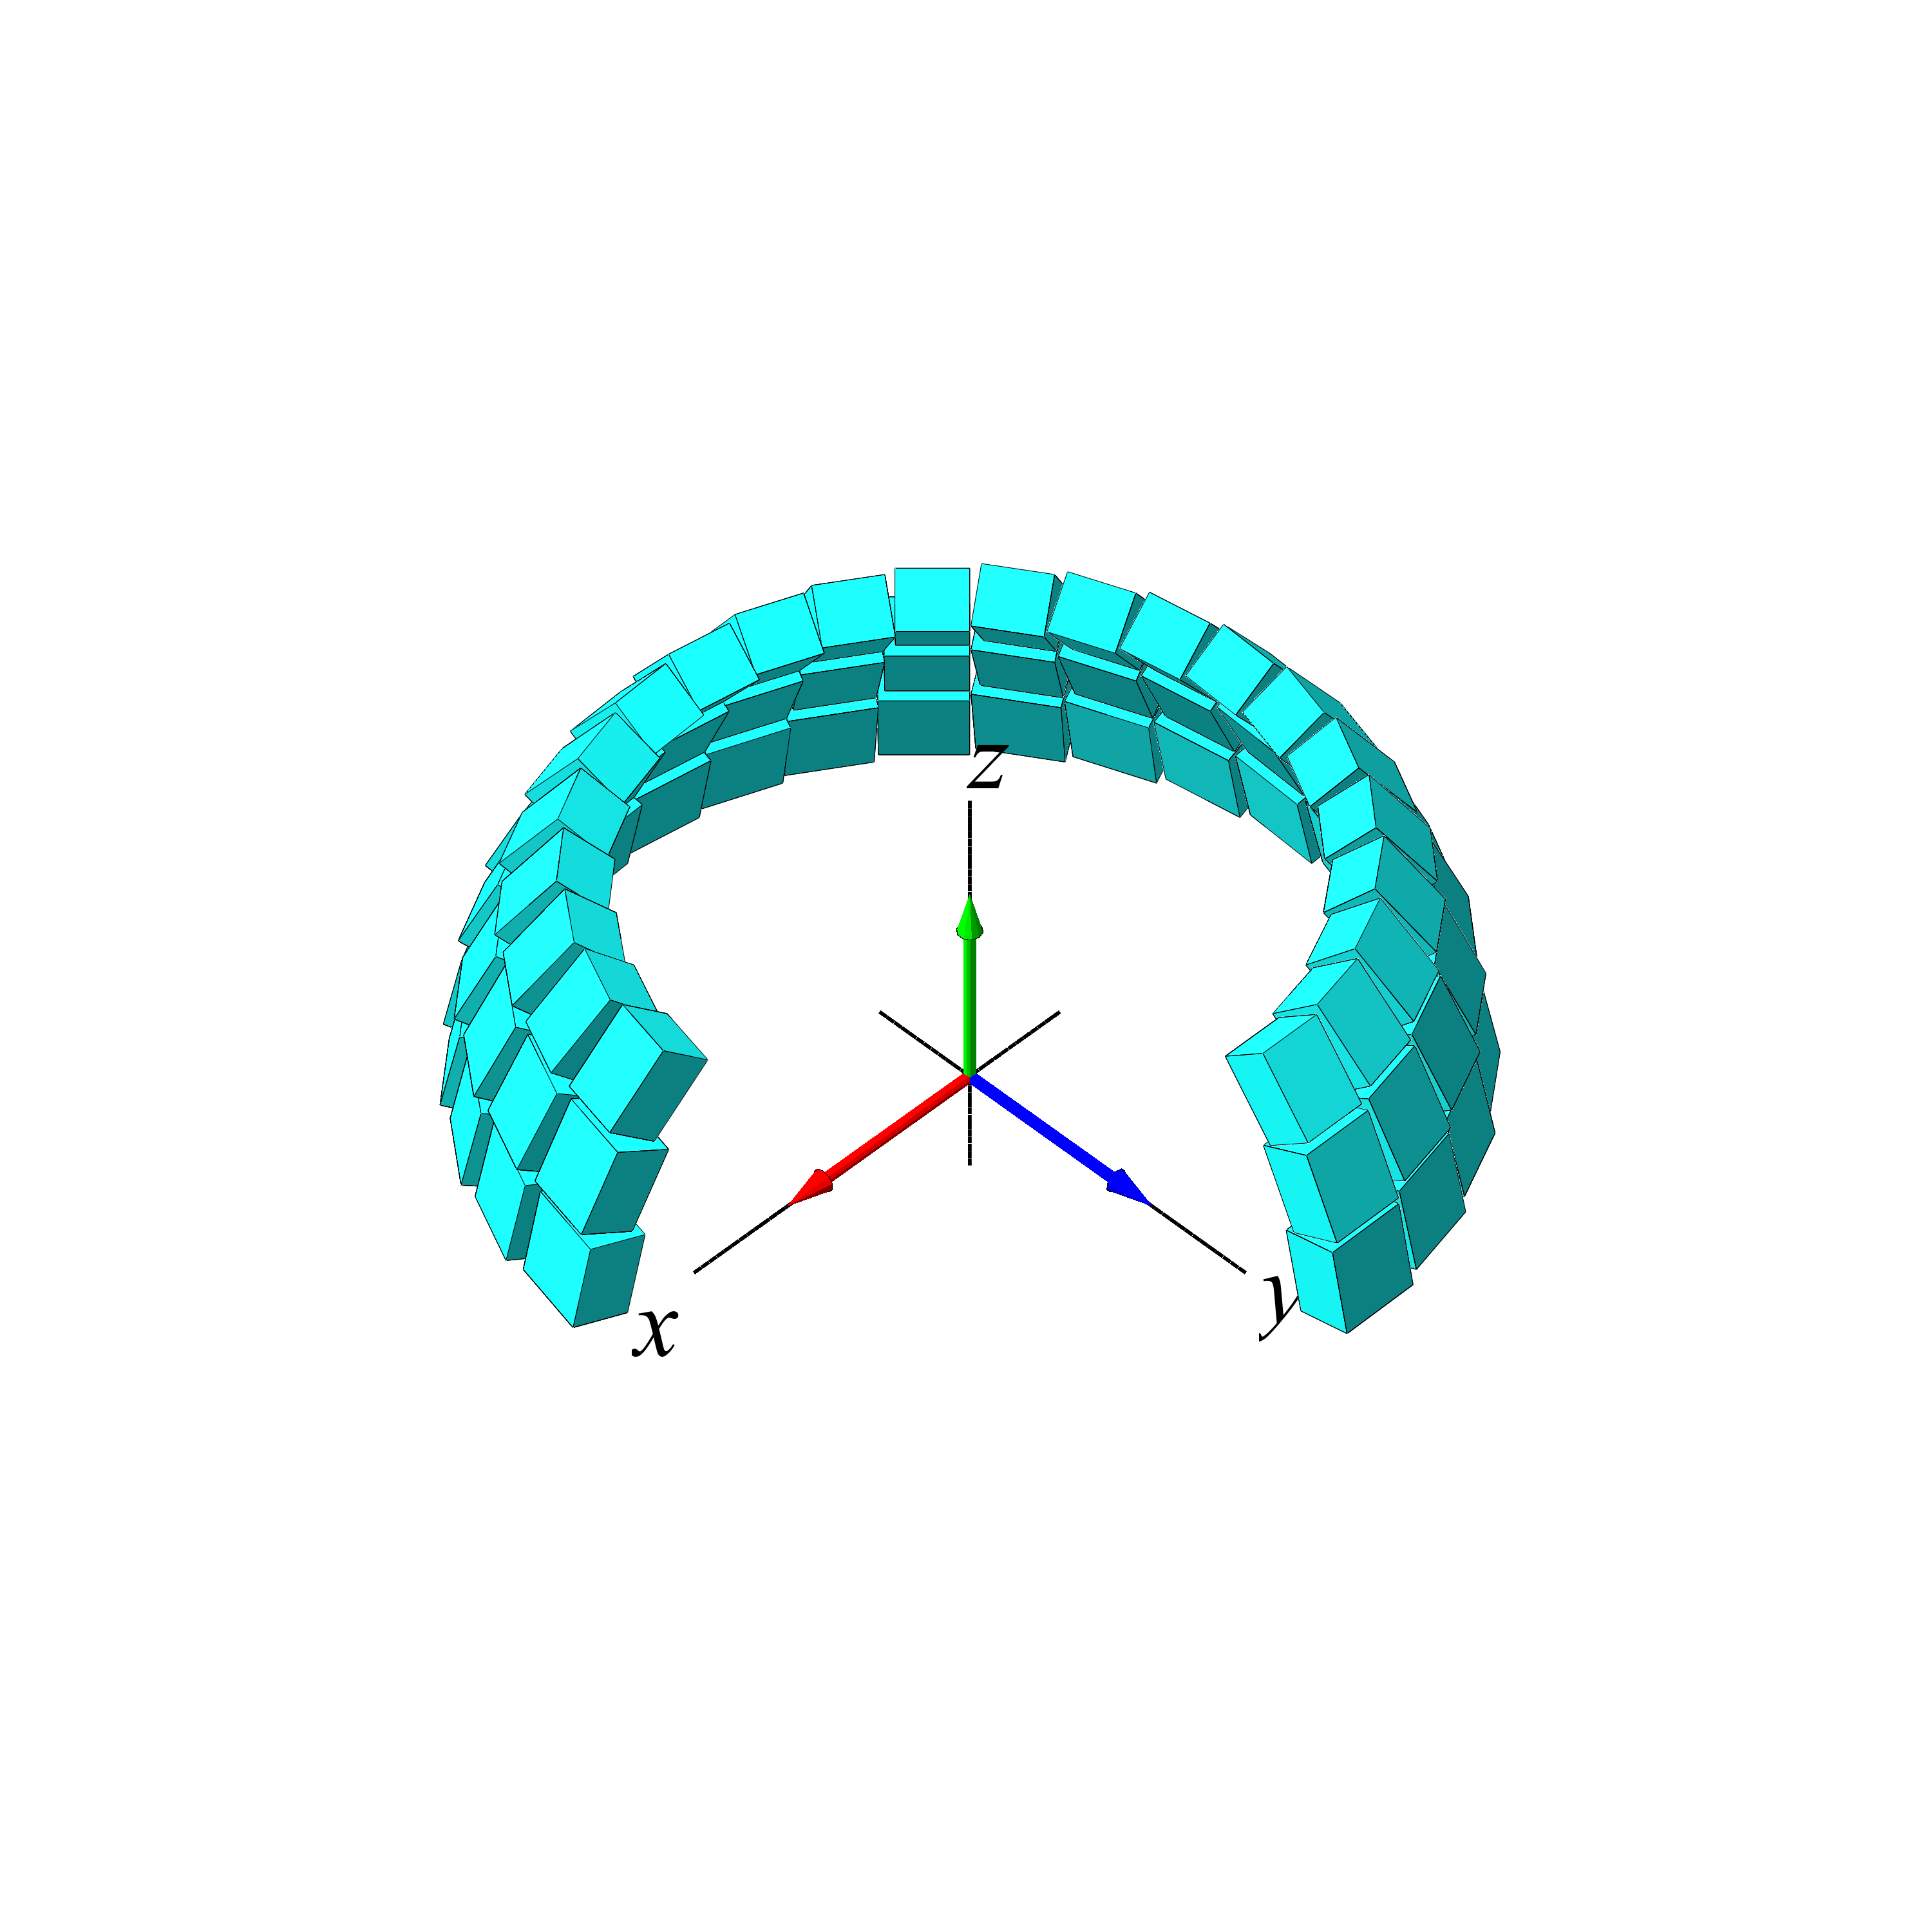
\includegraphics[height=80mm]{FIGS/plotKugleskal}}
\begin{center}
\caption{\small{Delvis opbygning af en  kugleskal.}} \label{figKugleskal}
\end{center}
\end{figure}




\begin{figure}[h]
\centerline{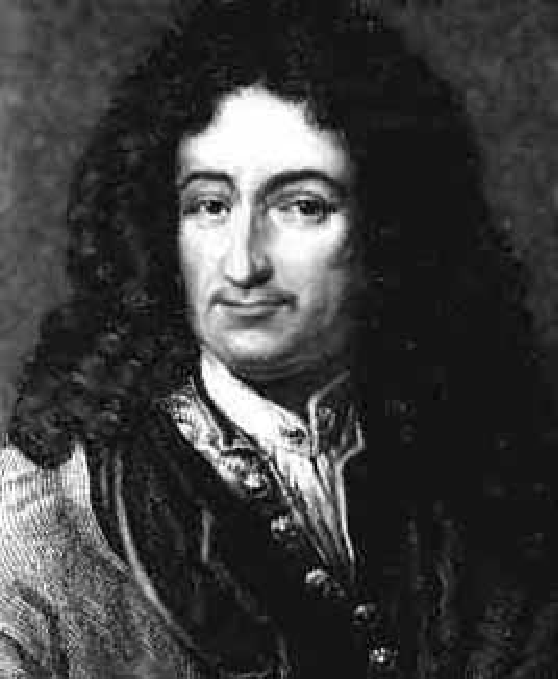
\includegraphics[height=50mm]{FIGS/PERSLeibniz} \qquad 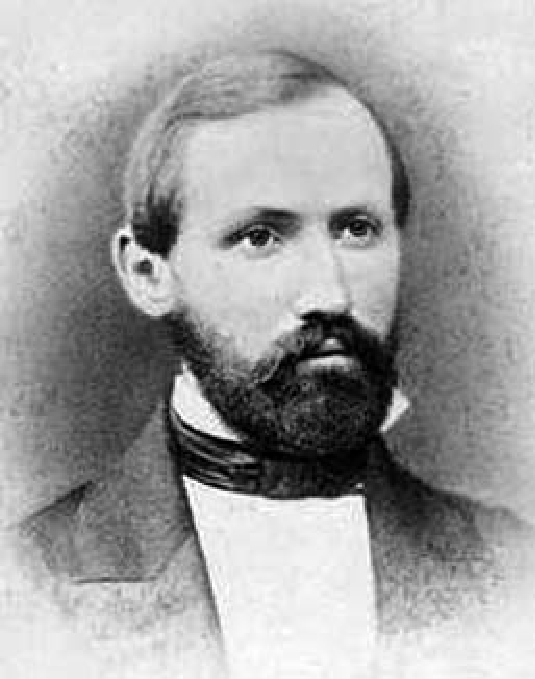
\includegraphics[height=50mm]{FIGS/PERSRiemann_3}}
\begin{center}
\caption{\small{Gottfried Wilhelm von Leibniz (til venstre) og  Georg Friedrich Bernhard Riemann. }} \label{figLeibniz}
\end{center}
\end{figure}



%%%%%%%%%%%%%%%%%%%%%%%%%%%%%%%%%%%%%%%%%%%%%%%%%%%%%%%%%%%%%%%%%%%%%%%%
%%%%%%%%%%%%%%%%%%%%%%%%%%%%%%%%%%%%%%%%%%%%%%%%%%%%%%%%%%%%%%%%%%%%%%%%


\section{Approksimerende {summer} og eksakte {integraler}} \label{secSummer}
På den reelle $u$-akse betragter vi en fast valgt kontinuert reel
funktion $f(u)$ på intervallet $[0,1]$, f.eks. $f(u)\,=\, 1+u+u^{2}$. For et givet helt tal $n >0$
gør vi nu følgende. Først deles intervallet $[0, 1]$ i $n$ lige
store delintervaller, som derved hver får længden $\,\delta_{u} \, =
\, \frac{1}{n}\, $. Delintervallernes venstre endepunkter har
$\,u-$koordinaterne:
$$
u_{1} = 0, \quad u_{2} = \frac{1}{n},\quad u_{3} = \frac{2}{n},\quad
u_{4} = \frac{3}{n},\cdots , \quad u_{n-1} = \frac{n-2}{n},\quad
u_{n} = \frac{n-1}{n} \quad .
$$
Det vil sige, at det $i$'te intervals venstre endepunkt har
$u-$koordinaten $\,u_{i}\, = \, (i-1)\,\frac{1}{n}\, = \,
(i-1)\,\delta_{u}\,$, hvor $\, i = 1, 2, 3, ..., n-1, n \,$.


\begin{exercise}
Bemærk, at hvis vi forøger antallet af delintervaller $\,n\,$ med
$1$, og nu ønsker en deling af $\,[0, 1]\,$ i $\, n+1 \, $ lige
store delintervaller, så vil alle de tidligere placerede $\,n\,$
venstre endepunkter i intervallet $[0, 1]$ skulle flyttes lidt
(pånær $u_{1}$) for at give plads til det ekstra delinterval. Hvor
meget?
\end{exercise}

For et fast antal delintervaller, $n$, finder vi
funktionsværdien af $f$ i hvert af
delintervallernes venstre endepunkter, altså de
$n$ værdier $f(0)$, $f(\frac{1}{n})$,
$f(\frac{2}{n})$, $f(\frac{3}{n})$, ...,
$f(\frac{n-1}{n})$.\\

Summen af disse værdier vil sædvanligvis afhænge meget af antallet
$\,n\,$ af funktionsværdier, men hvis vi først ganger hver enkelt
funktionsværdi med delinterval-længden  $\delta_{u}$ får vi følgende såkaldte  \emph{vægtede sum} af
funk\-tions\-vær\-di\-er\-ne, som iøvrigt derved netop er en approksimation til det med fortegn
regnede areal af området imellem $u-$aksen og grafen for $f(u)$ over intervallet (jvf. figur \ref{FigIS}):
\begin{equation} \label{eqIntSum}
\operatorname{I}(f, n, [0,1]) = \sum_{i=1}^{i=n}\,
f\left((i-1)\frac{1}{n}\right)\,\frac{1}{n} \, = \,
\sum_{i=1}^{i=n}\, f\left((i-1)\delta_{u}\right)\,\delta_{u} \, = \,
\sum_{i=1}^{i=n}\, f\left(u_{i}\right)\,\delta_{u} \quad .
\end{equation}



\begin{exercise}
Vis, at den vægtede sum af funktionsværdierne af $f$ i ligning
(\ref{eqIntSum}) er opadtil begrænset  af $f$'s største værdi og nedadtil begrænset af $f$'s
mindste værdi i intervallet $[0,1]$.
\end{exercise}

Den vægtede sum er ikke blot begrænset for alle
$\,n\,$. Det viser sig nemlig, at den også har en grænseværdi for $\,n\,$
gående imod  uendelig -- i hvert fald hvis $f(u)$ er kontinuert; det er den grænseværdi vi
kalder Riemann-integralet af $\,f(u)\,$ over intervallet
$\,[0,1]\,$ (efter B. Riemann, se figur \ref{figLeibniz}).
Selve grænseværdien {\emph{betegnes}} (efter G. Leibniz, se figur \ref{figLeibniz}) med følgende notation
\begin{equation} \label{eqRiemannSum}
\lim_{n \to \infty} \operatorname{I}(f,n, [0, 1]) \, = \, \int_{0}^{1} f(u)\, du \quad .
\end{equation}



\begin{figure}[h]
\centerline{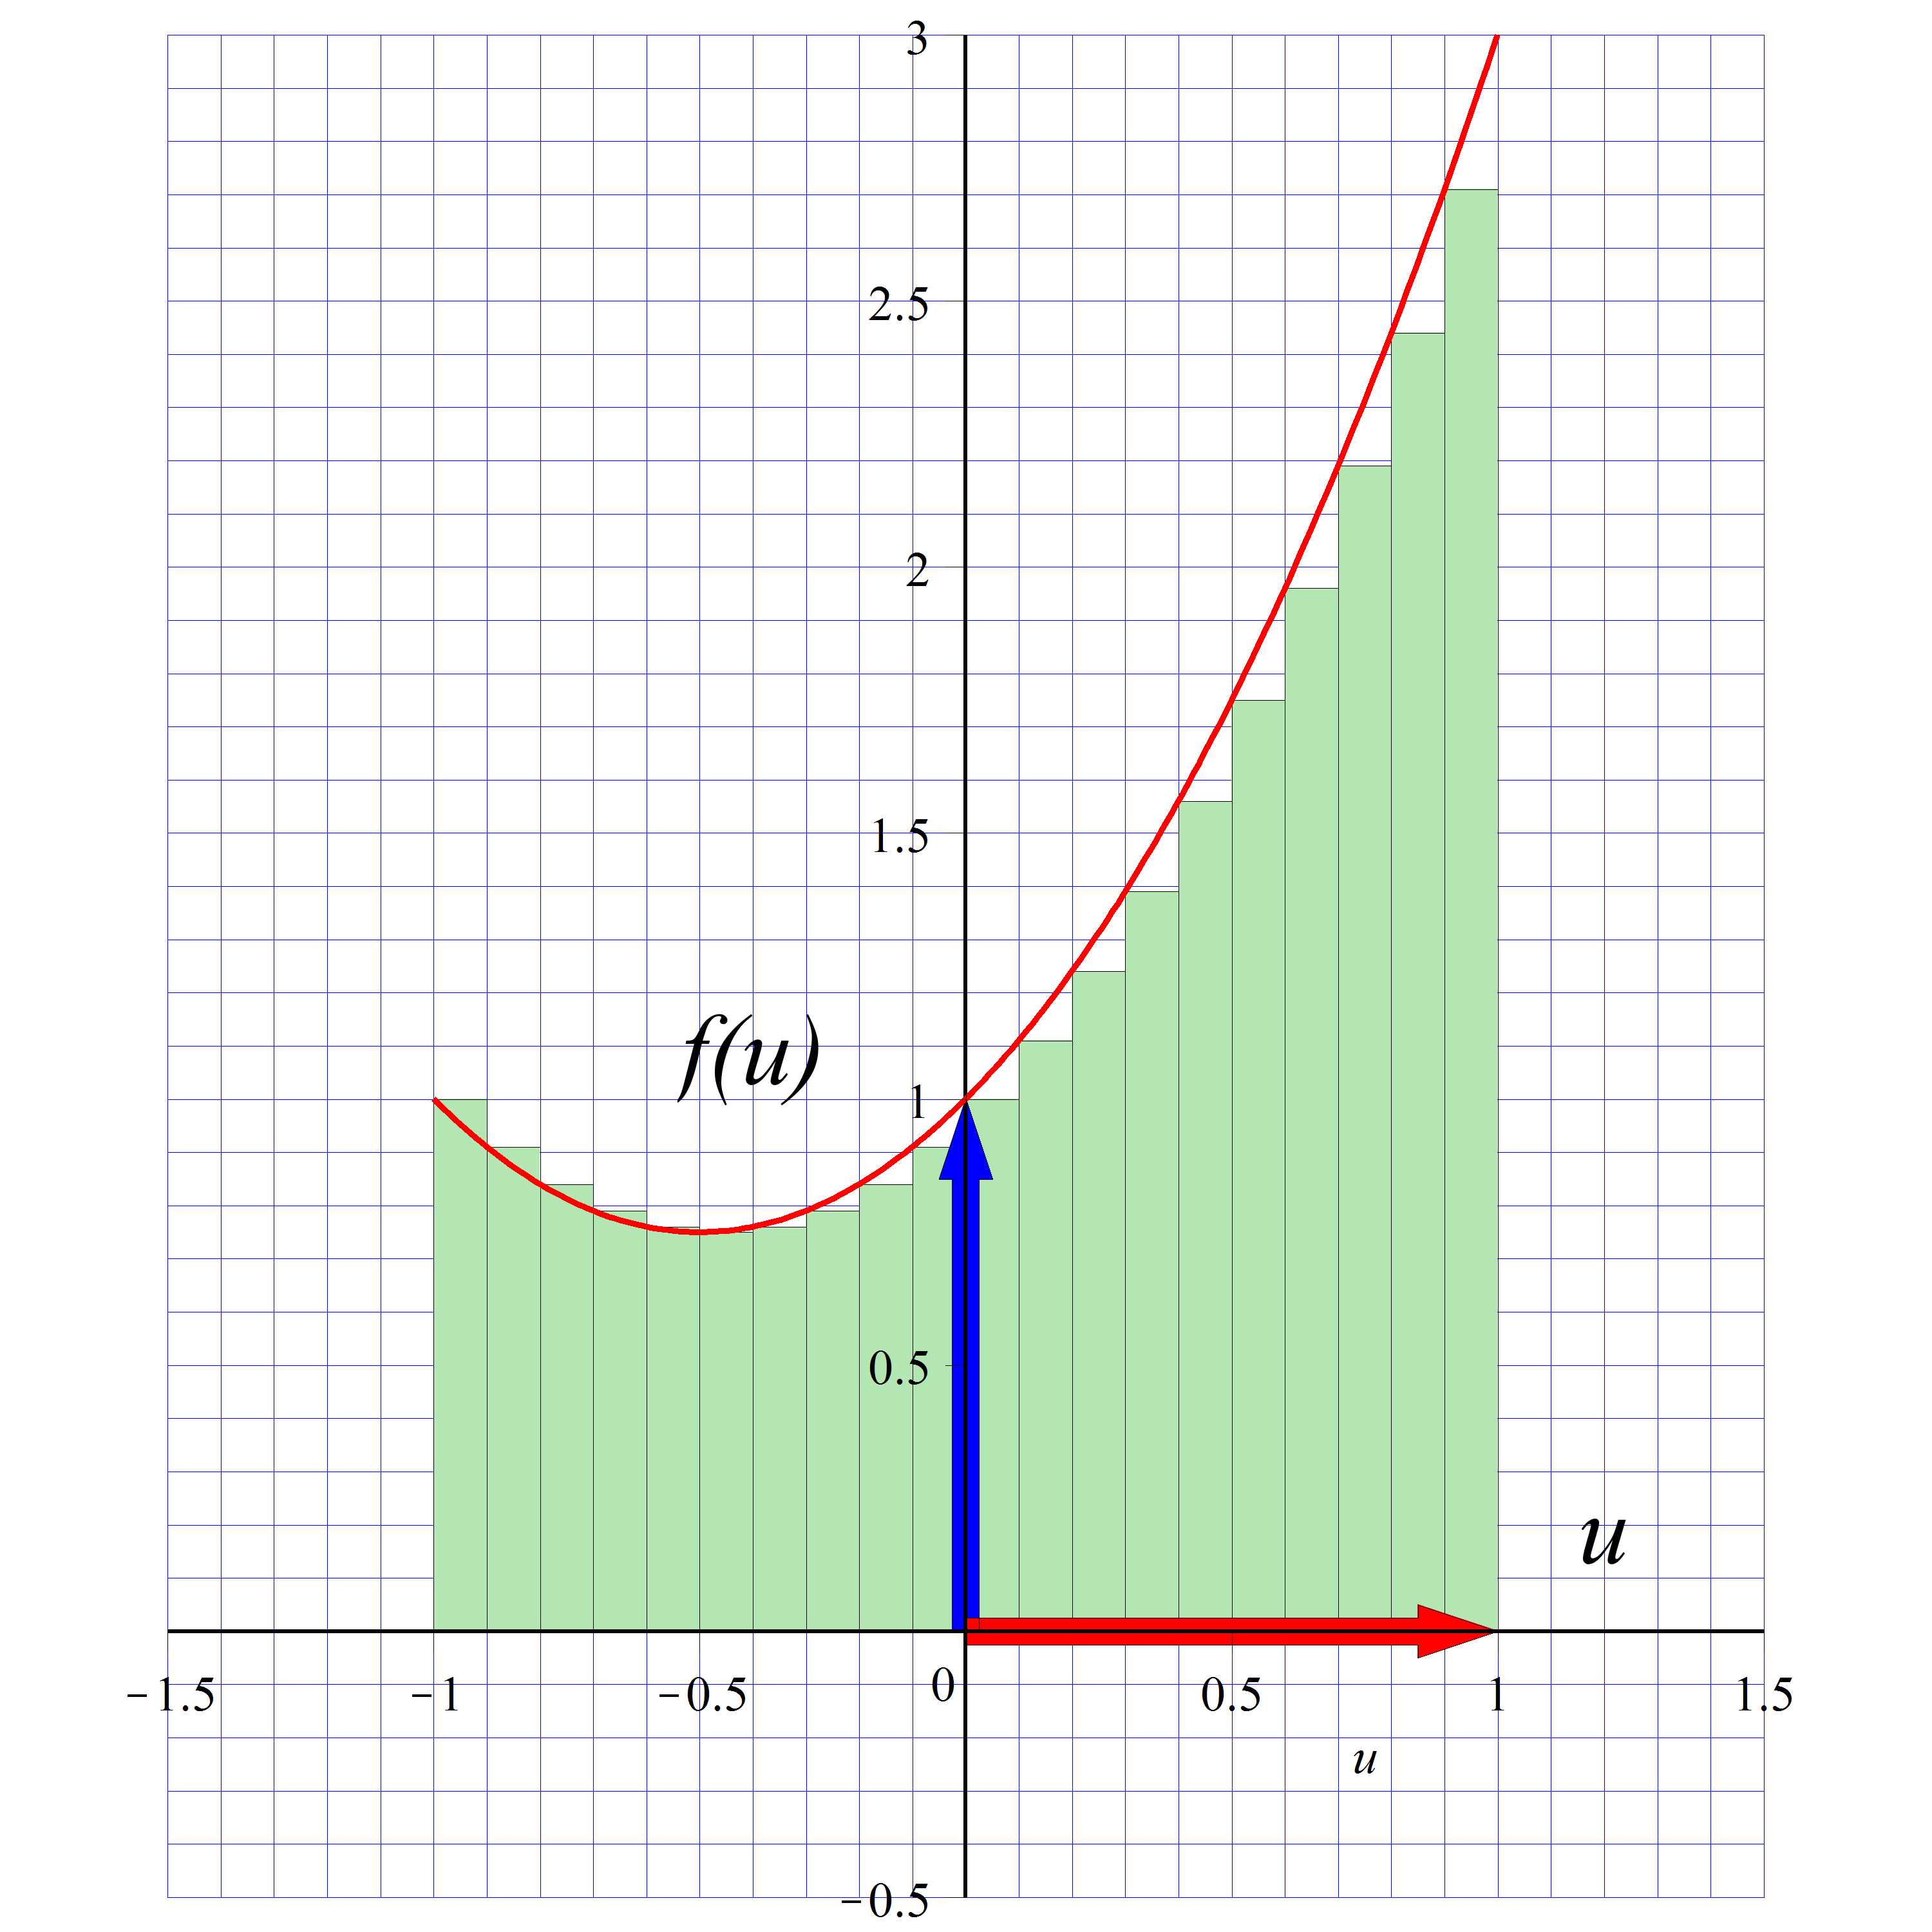
\includegraphics[height=90mm]{FIGS/plotIntArea}}
\begin{center}
\caption{\small{Figuren viser areal-repræsentationen
af integralsummen $\operatorname{I}(f,n, [-1,1])$ for funktionen $\,f(u) \, = \, 1 + u
+ u^{2}\,$  (se opgave
\ref{exIS2}) med $\,n = 20\,$ delintervaller i
intervallet $\,[a, b] = [-1, 1]\,$. De $20$
addender i summen er repræsenteret ved
rektangulære søjler med den fælles bredde
$(b-a)/20 = 1/10$ og højder givet ved værdierne
af funktionen $f(u) = 1 + u + u^2$ i
delin\-ter\-vallernes venstre endepunkter. }}
\label{FigIS}
\end{center}
\end{figure}





\begin{example}[Konstant funktion]\label{exampConst}
Lad $f(u) = \alpha$ for alle $u\in [0,1]$, hvor $\alpha$ er en konstant. Så er
\begin{equation}
\begin{aligned}
\operatorname{I}(f,n, [0, 1]) &= \sum_{i=1}^{i=n}\, f\left(u_{i}\right)\,\delta_{u} \\
&= \sum_{i=1}^{i=n}\, \alpha \cdot \frac{1}{n} \\
&= \frac{\alpha}{n} \cdot \sum_{i=1}^{i=n}\, 1 \\
&= \frac{\alpha}{n} \cdot n \\
&= \alpha \quad ,
\end{aligned}
\end{equation}
således at
\begin{equation}
\lim_{n \to \infty} \operatorname{I}(f,n, [0, 1]) \, = \, \int_{0}^{1} \alpha \, du = \alpha \quad .
\end{equation}
\end{example}

\begin{example}[Førstegradspolynomium]\label{exampLin}
Lad $f(u) = \alpha + \beta\cdot u$ for $u\in [0,1]$, hvor $\alpha$ og $\beta$ er konstanter. Det vil sige at grafen for $f(u)$ er et ret linjestykke over intervallet  $u\in [0,1]$ på $u$-aksen. Så er
\begin{equation}
\begin{aligned}
\operatorname{I}(f,n, [0, 1]) &= \sum_{i=1}^{i=n}\, f\left(u_{i}\right)\,\delta_{u} \\
&= \sum_{i=1}^{i=n}\, \left(\alpha + \beta\cdot u_{i}\right) \cdot \frac{1}{n} \\
&= \sum_{i=1}^{i=n}\, \left(\alpha + \beta\cdot (i-1)\cdot \frac{1}{n}\right) \cdot \frac{1}{n} \\
&= \alpha \cdot \left(\sum_{i=1}^{i=n}\, \frac{1}{n}\right) + \beta\cdot \left(\sum_{i=1}^{i=n}\,(i-1)\cdot \frac{1}{n^{2}}\right)\\
&= \alpha + \beta\cdot \sum_{i=1}^{i=n}\,\frac{i}{n^{2}} - \beta\cdot \sum_{i=1}^{i=n}\,\frac{1}{n^{2}}\\
&= \alpha + \beta \cdot \frac{1}{n^{2}}\sum_{i=1}^{i=n}\,i - \beta\cdot \frac{1}{n} \quad ,
\end{aligned}
\end{equation}
hvor vi så har brug for følgende identitet:
\begin{equation}
\frac{1}{n^{2}}\sum_{i=1}^{i=n}\,i = \frac{1}{n^{2}}\cdot \frac{(n+1)\cdot n}{2} =  \frac{(n+1)}{2\cdot n} \quad ,
\end{equation}
sådan at
\begin{equation}
\operatorname{I}(f,n, [0, 1]) = \alpha + \beta \cdot \frac{(n+1)}{2\cdot n} - \beta\cdot \frac{1}{n} \quad .
\end{equation}
Det følger heraf, at
\begin{equation}
\lim_{n \to \infty} \operatorname{I}(f,n, [0, 1]) \, = \, \alpha + \beta \cdot \frac{1}{2} \quad , 
\end{equation}
og dermed 
\begin{equation}
\int_{0}^{1} \alpha + \beta \cdot u   \, du \, = \, \alpha +  \frac{1}{2} \cdot \beta \quad .
\end{equation}


Bemærk, at den fundne værdi er præcis arealet af området imellem grafen for $f(u) = \alpha + \beta\cdot u$ og $u$-aksen over intervallet $[0, 1]$ for så vidt grafen der ligger helt over $u$-aksen.

\end{example}


Hvis vi benytter den samme strategi som ovenfor, men nu med en deling
af det mere generelle interval $\,[a, b]\,$ på
$\,u\,$-aksen i $\,n\,$ lige store
delintervaller, har vi følgende sætning:

\begin{theorem}[Integralsum og Riemann-integral]\label{thmInt}
Lad $f(u)$ betegne en kontinuert funktion på intervallet $[a,b]$.
For ethvert $n$ inddeles intervallet i $n$ lige store
delintervaller, hver med længden $\,\delta_{u} = (b-a)/n\,$. Disse
delintervallers venstre endepunkter har så koordinaterne $\,u_{i} =
a + (i-1)\delta_{u}\,$ for $\, i = 1, 2, 3, ..., n-1, n \,$. Lad
$\,\operatorname{I}(f, n, [a,b])\,$ betegne følgende sum:
\begin{equation} \label{eqIS1}
\begin{aligned}
 \operatorname{I}(f, n, [a,b]) &= \sum_{i=1}^{i=n}\, f\left(a+
(i-1)\frac{b-a}{n}\right)\,\left(\frac{b-a}{n}\right) \\
&= \sum_{i=1}^{i=n}\, f\left(a+
(i-1)\delta_{u}\right)\,\delta_{u} \,
= \,
\sum_{i=1}^{i=n}\, f\left(u_{i}\right)\,\delta_{u} \quad .
\end{aligned}
\end{equation}
Så har  $\operatorname{I}(f,n, [a, b])$ en grænseværdi for $n$ gående imod $\infty$. Grænseværdien kaldes \ind{Riemann-integralet}{Riemann-integralet} af $f(u)$ over $[\,a,\, b\,]$ og betegnes med $\int_{a}^{b} f(u)\, du$:
\begin{equation}
\operatorname{I}(f,n, [a, b]) =  \sum_{i=1}^{i=n}\, f\left(u_{i}\right)\,\delta_{u} \to \int_{a}^{b} f(u)\, du \quad \rm{for}\quad  n \to \infty\quad.
\end{equation}
\end{theorem}


\begin{exercise}
Lad $f(u) = \alpha + \beta\cdot u$ for givne konstanter $\alpha$ og $\beta$ og lad $[a, b]$ betegne et interval på $u$-aksen. Bestem for ethvert $n$ værdien af
\begin{equation}
 \operatorname{I}(f,n, [a,b]) \quad ,
\end{equation}
find dernæst grænseværdien
\begin{equation}
\lim_{n \to \infty} \operatorname{I}(f,n, [a,b]) \quad ,
\end{equation}
og sammenlign med arealet af området mellem (den retlinjede) grafen for $f(u)$ og $u$-aksen.
\end{exercise}


Summer af typen $\,\operatorname{I}(f, n, [a,b])\,$ vil vi
i det følgende kalde
\ind{integralsummer}{integralsummer}.
Det er eksistensen af grænseværdier af disse integralsummer, der er det helt afgørende for vort forehavende. Bemærk for eksempel, at
grænseværdien $\int_{a}^{b} f(u)\, du$ jo nu er det bedste bud på, hvad vi skal forstå ved arealet af det plane  område
imellem $u-$aksen og grafen for $f(u)$ over intervallet $[a, b]$ (for så vidt at $f(u)$ er positiv i hele intervallet).
I opgave \ref{exIS2} og i eksemplerne \ref{exampSinusSum} og \ref{exampFresnelC} behandles andre eksempler på, hvordan sådanne grænseværdier (og arealer) kan beregnes direkte ud fra en analyse af, hvordan summerne $\sum_{i=1}^{i=n}\, f\left(u_{i}\right)\,\delta_{u}$ opfører sig når $n \to \infty$.\\

\begin{aha}
Bemærk, at
Riemann-integralet netop konstrueres og opstår som en uendelig sum af uendeligt små addender $\sum_{i=1}^{i=n}\, f\left(u_{i}\right)\,\delta_{u}$ for $n \to \infty\,$, altså
præcis som vi havde brug for det i forbindelse med vore overvejelser om rumfanget af kuglen ovenfor
og i figur \ref{figSphereFill}.
\end{aha}





%%%%%%%%%%%%%%%%%%%%%%%%%%%%%%%%%%%%%%%%%%%%%%%%%%%%%%%%%%%%%%%%%%%%%%%%
%%%%%%%%%%%%%%%%%%%%%%%%%%%%%%%%%%%%%%%%%%%%%%%%%%%%%%%%%%%%%%%%%%%%%%%%



\section{Stamfunktionsbestemmelse} \label{secStamfunk}
Riemann-integraler kan bestemmes ved hjælp af stamfunktioner -- det er præcis indholdet af den fundamentalsætning, som vi vil formulere og bruge i næste afsnit. Vi vil antage i det følgende,
at vi allerede for passende elementære funktioner $f(x)$
er i stand til at finde stamfunktionerne $F(x)$ til $f(x)$. Som bekendt går det ud på at finde alle de
funktioner $F(x)$ der opfylder, at $F'(x) \,= \, f(x)$. De funktioner  betegner vi som følger ved hjælp af \ind{integraltegnet}{integraltegnet}, og vi siger, at \ind{integranden}{integranden} $f(x)$ {\emph{integreres}} og giver {\emph{integralet}} eller \emph{stamfunktionen} $F(x)$:
\begin{equation}
F(x) \, = \, \int \, f(x)\,dx \quad .
\end{equation}
Hvis $F(x)$ er en stamfunktion til $f(x)$ og $c$ en reel konstant, så er $F(x) + c$ også en stamfunktion til $f(x)$. Og {\emph{alle}} stamfunktionerne til $f(x)$ fås ved at finde \'{e}n stamfunktion og dertil lægge vilkårlige (arbitrære) konstanter $c$. \\

Her er nogle eksempler på stamfunktioner til nogle velkendte funktioner $f(x)$ (vi angiver kun \'{e}n stamfunktion til hver af de givne funktioner):


\begin{equation}
\begin{aligned}
f(x) \, = \, a \quad , \quad F(x) \, &= \, \int  f(x) \,dx \, = \, ax\\
f(r) \, = \, 4\pi r^{2} \quad , \quad F(r) \,&= \, \int  f(r) \,dr \, = \, \dfrac{4}{3}\pi r^{3}\\
f(t) \, = \, 1/(1+t^{2}) \quad , \quad F(t) \,&= \, \int  f(t) \,dt \, = \, \arctan(t)\\
f(u) \, = \, 1 + u + u^{2} \quad , \quad F(u) \,&= \, \int  f(u) \,du \, = \, u +
\dfrac{1}{2}u^{2} + \dfrac{1}{3}u^{3}\\
f(x) \, = \, \sin(x^{2}) \quad , \quad F(x) \,&= \, \int  f(x) \,dx \, = \, \sqrt{\frac{\pi}{2}}\cdot \operatorname{FresnelS}\left(x\cdot \sqrt{\frac{2}{\pi}}\right)\\
f(x) \, = \, \e^{-x^{2}} \quad , \quad F(x) \,&= \, \int  f(x) \,dx \, = \, \frac{1}{2}\sqrt{\pi}\,\operatorname{erf}(x) \\
f(x) \, = \, \e^{x} \quad , \quad F(x) \,&= \, \int  f(x) \,dx \, = \, \e^{x}   \quad .
\end{aligned}
\end{equation}

Da vi i de eNoter der handler om integration i flere variable har udstrakt brug for at kunne finde stamfunktioner -- også for lidt mere indviklede integrand-funktioner -- nævner vi følgende to sætninger, der kan være en hjælp til omformning af givne stamfunktionsproblemer til bestemmelse af simplere stamfunktioner.

\begin{theorem}[Partiel integration]\label{thmPartielInt}
Lad $f(x)$ betegne en kontinuert funktion med en stamfunktion $F(x)$ og lad $g(x)$ være en differentiabel funktion med kontinuert afledet $g'(x)$. Så kan alle stamfunktioner til produktet $f(x)\cdot g(x)$ bestemmes ved:
\begin{equation}\label{eqPartielRegel}
\int f(x)\cdot g(x) \, dx = F(x)\cdot g(x) - \int  F(x)\cdot g'(x) \, dx.
\end{equation}
\end{theorem}
\begin{bevis}
Vi skal blot vise, at de to sider af ligningen (\ref{eqPartielRegel}) har samme differentialkvotienter for alle $x$! To funktioner er stamfunktioner for den samme integrandfunktion, hvis deres differens er en konstant. De afledede er ens fordi:
\begin{equation}
\begin{aligned}
\frac{d}{dx}\left(\int\, f(x)\cdot g(x) \, dx\right) &= f(x)\cdot g(x) \\ \\
\frac{d}{dx}\left( F(x)\cdot g(x) - \int F(x)\cdot g'(x) \, dx \right) &= F'(x)\cdot g(x) + F(x)\cdot g'(x) -  F(x)\cdot g'(x)\\
&=  f(x)\cdot g(x) \quad .
\end{aligned}
\end{equation}
\end{bevis}

\begin{example}[Partiel integration] \label{exampPartielInt}
Vi vil bestemme en stamfunktion til $h(x) = x\cdot \sin(x)$. Først skriver vi $h(x) = f(x)\cdot g(x)$ med $f(x)= \sin(x)$ og $g(x) = x$. Så har vi i henhold til reglen om partiel integration:
\begin{equation}
\int\,x\cdot \sin(x) \, dx = x\cdot (-\cos(x)) - \int\, 1 \cdot (-\cos(x))\, dx = - x\cdot \cos(x) + \sin(x) \quad .
\end{equation}
\end{example}

\begin{exercise} \label{exercCosSin}
Bestem samtlige stamfunktioner til funktionen $f(x) = \cos(x)\cdot \sin(x)$.
\end{exercise}


\begin{theorem}[Integration ved substitution]\label{thmSubstitutInt}
Lad $f(x)$ være en kontinuert funktion og lad $g(u)$ betegne en monoton, differentiabel funktion med kontinuert afledet $g'(u)$. Så  kan vi bestemme en stamfunktion til $f(x)$ ved hjælp af den sammensatte funktion $f(g(u))$ således:
\begin{equation}\label{eqSubstRegel}
\int\,f(x) \, dx = \left( \int \, f(g(u))\cdot g'(u) \, du \right)_{u = g^{\circ - 1}(x)} \quad ,
\end{equation}
hvor $g^{\circ - 1}(x)$ betegner den omvendte funktion til $g(u)$.
\end{theorem}
\begin{bevis}
Vi skal igen vise, at de to sider i (\ref{eqSubstRegel}) har samme differentialkvotient for alle $x$:
\begin{equation}
\begin{aligned}
\frac{d}{dx}\left( \int\,f(x) \, dx \right) &= f(x) \quad  \textrm{og} \\ \\
\frac{d}{dx}\left(\int \, f(g(u))\cdot g'(u) \, du \right)_{u = g^{\circ - 1}(x)} \\
&= \frac{d}{du}\left(\int \, f(g(u))\cdot g'(u) \, du \right)_{u = g^{\circ - 1}(x)} \cdot \frac{d}{dx}\left( g^{\circ - 1}(x)\right) \\
&= \left( f(g(u))\cdot g'(u)\right)_{u = g^{\circ - 1}(x)} \cdot \frac{1}{g'(u)} \\
&= f(g(u)) \\
&= f(x) \quad ,
\end{aligned}
\end{equation}
hvor vi undervejs har benyttet reglen om differentiation af sammensatte funktioner (kædereg\-len) og reglen om differentiation af omvendte funktioner, se \tref{NUID27-tn14}{eNote}.
\end{bevis}

\begin{example}[Substitution]\label{exampSubst}
Vi vil bestemme en stamfunktion til funktionen
\begin{equation}
f(x) = \frac{\sqrt{x}}{1+x} \quad , \quad x \in \, ]0, \infty[\,
\end{equation}
altså:
\begin{equation}
\int\,f(x) \, dx  = \int\,\frac{\sqrt{x}}{1+x} \, dx .
\end{equation}
Hvis vi substituerer med funktionen $g(u) = u^{2}$ for $u \in \, ]0, \infty[ \, $ får vi 'fjernet' kvadratrodstegnet og har dermed ingredienserne til brug i substitutionsreglen:
\begin{equation}
\begin{aligned}
f(g(u)) &= \frac{u}{1+u^{2}} \\
g'(u) &= 2\cdot u \quad .
\end{aligned}
\end{equation}
Vi indsætter og får:
\begin{equation}
\begin{aligned}
\int\,f(x) \, dx  &= \int\,\frac{\sqrt{x}}{1+x} \, dx \\
&= \left( \int \,\frac{u}{1+u^{2}}\cdot 2\cdot u \, du \right)_{u = g^{\circ -1}(x)} \\
&= \left( \int \,2\cdot \frac{u^{2} + 1 - 1}{1+u^{2}} \, du \right)_{u = \sqrt{x}} \\
&= 2\cdot\left( \int \, \left(1 - \frac{1}{1+u^{2}} \right)\, du \right)_{u = \sqrt{x}} \\
&= 2 \cdot \left( u - \arctan(u) \right)_{u = \sqrt{x}} \\
&= 2\cdot \left( \sqrt{x} - \arctan(\sqrt{x}) \right) \quad , \quad x \in \, ]0, \infty[ \quad .
\end{aligned}
\end{equation}
\end{example}

\begin{exercise} \label{exercExp2}
Bestem samtlige stamfunktioner til funktionen $f(x) = x\cdot\e^{x^{2}}$.
\end{exercise}


%%%%%%%%%%%%%%%%%%%%%%%%%%%%%%%%%%%%%%%%%%%%%%%%%%%%%%%%%%%%%%%%%%%%%%%%
%%%%%%%%%%%%%%%%%%%%%%%%%%%%%%%%%%%%%%%%%%%%%%%%%%%%%%%%%%%%%%%%%%%%%%%%


\section{Fundamental-sætningen}\label{secFundamI}


Følgende fundamentale sætning etablerer den antydede relation mellem stamfunktionsbestemmelse og Riemann-integralerne, og det er den vi benytter os kraftigt af i de eNo\-ter, der handler om integration i flere variable.

\begin{theorem}[Integralregningens fundamentalsætning]\label{thmAnalyseFundamental}
Lad $f(u)$ betegne en kontinuert funktion på intervallet $[a, b]$. Antag, at $F(u)$ er en (vilkårlig) stamfunktion for $f(u)$.
Så gælder følgende:
\begin{equation}
\lim_{n \to \infty} \operatorname{I}(f,n, [a, b]) \, = \, \int_{a}^{b}\,f(u) \,du \, = \, [\, F(u)\, ]_{u=a}^{u=b}\,\,\, = \, F(b) - F(a) \quad .
\end{equation}
\end{theorem}

\begin{aha}
Vi vil ikke her bevise fundamentalsætningen -- blot bemærke, at man godt kan forvente, at stamfunktionen til $f(u)$ kan
give integralsummens grænseværdi som i sætning \ref{thmAnalyseFundamental}: Hvis vi for et givet $n$ lader
\begin{equation}
\widehat{F}(x_{0}) = \operatorname{I}(f,n, [a, x_{0}])
\end{equation}
og hvis vi sætter $x_{0} = u_{n+1}$ og $x = x_{0} + \delta_{u}$, så er
\begin{equation} \label{eqBevFundam}
\begin{aligned}
\widehat{F}(x) &= \operatorname{I}(f,n+1, [a, x]) \\
&=  \operatorname{I}(f,n, [a, x_{0}]) + f(u_{n+1}) \cdot \delta_{u} \\
&= \widehat{F}(x_{0}) + f(x_{0}) \cdot (x-x_{0}) \quad ,
\end{aligned}
\end{equation}
Hvis vi et øjeblik tillader os at se bort fra $n$-afhængighederne og de nødvendige involverede grænseværdier for $n \to \infty$, så 'følger' det af (\ref{eqBevFundam}), at $\widehat{F}(x)$ er 'dif\-fe\-ren\-tiabel' i
$x_{0}$ med 'differentialkvotienten' $f(x_{0})$, se definitionen på differentiabilitet af en funktion af \'{e}n variabel i \tref{NUID27-tn14}{eNote},  \tref{NUID27-tn14.secDifferentiation}{afsnit}. I den forstand må vi forvente, at  $\widehat{F}(x)$ faktisk er en 'stamfunktion' til $f(x)$. Denne grove overvejelse er naturligvis kun en pejling i retning af et egentligt bevis for fundamentalsætningen.
\end{aha}


\begin{think}
Riemann-integralerne kan herefter beregnes på to måder, dels som grænseværdi af integralsummer
og dels som en differens mellem evalueringerne af en stam\-funk\-tion i interval-endepunkterne.
Det er sædvanligvis den sidste metode, det er smartest at benytte sig af, hvis altså
de relevante stamfunktioner kan findes eller bestemmes.
\end{think}


\begin{figure}[h]
\centerline{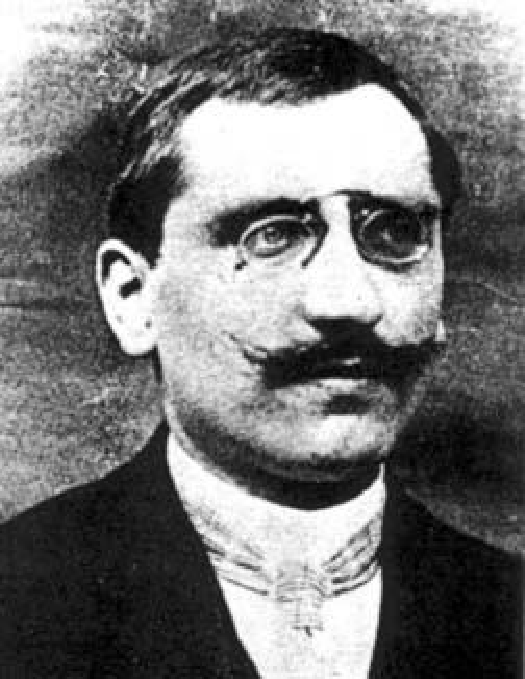
\includegraphics[height=50mm]{FIGS/PERSLebesgue} \qquad  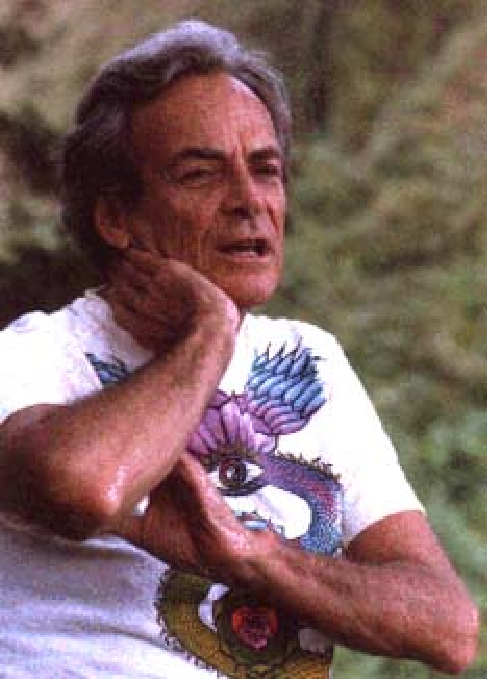
\includegraphics[height=50mm]{FIGS/PERSFeynman_8}
\qquad 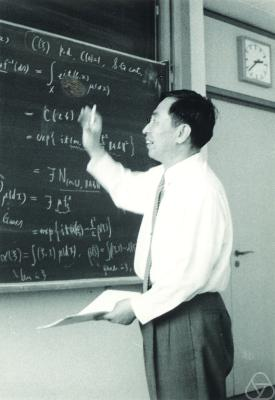
\includegraphics[height=50mm]{FIGS/PERSIto}}
\begin{center}
\caption{\small{Henri L\'{e}on Lebesgue, Richard P. Feynman,
og Kiyosi Ito.}} \label{figLebesgueItoFeynman}
\end{center}
\end{figure}

\begin{info}
Riemann-integration er senere blevet udviklet betydeligt til gavn for og brug i adskillige anvendelser. Lebesgue's integral- og målteori fra 1901 gør det for eksempel muligt at udvide begreberne længde, areal, og volumen til også at give konsistent mening for f.eks. fraktale geometriske objekter. Ito-calculus, Santalo's integralgeometri, og Feynman's sti-integraler er blandt de nyeste udviklinger med spændende anvendelser i så vidt forskellige discipliner som finansiel matematik og kvantefeltteori.
\end{info}


Vi illustrerer her fundamentalsætningen og de to beregningsmetoder i form af en opgave og et par eksempler:






\begin{exercise} \label{exIS2}
Lad $f(u) = 1 + u + u^{2}$, $\,u \in [-1, 1]\,$. Så er
\begin{equation}\label{eqexIS2}
\begin{aligned}
\operatorname{I}(f,n, [-1,1]) \, & = \, \,  \sum_{i=1}^{i=n}\, \left(1 +
\left(-1+ (i-1)\frac{2}{n}\right) + \left(-1+
(i-1)\frac{2}{n}\right)^{2}
\,\right)\frac{2}{n} \\
 & = \, \, \sum_{i=1}^{i=n}\, \left(\frac{ 8 + 4\,n + 2\,n^{2} - 16\,i - 4\,i\,n + 8\,i^{\,2}}{n^{3}}\,\right) \,
  \quad .
\end{aligned}
\end{equation}
Benyt tabellen over del-summerne nedenfor til at beregne summen i (\ref{eqexIS2}) som funktion af $n$ og
dernæst til at eftervise
\begin{equation}\label{eqexIS2B}
\lim_{n \to \infty} \operatorname{I}(f,n, [-1,1]) = \int_{-1}^{1}
\left(\,1+u+u^{2}\,\right)\, du = F(1) - F(0) = \frac{8}{3}
 \quad ,
\end{equation}
idet en stamfunktion til $f(u)$ i dette tilfælde jo er $F(u) = u + \frac{1}{2}u^{2} + \frac{1}{3}u^{3}$ således at
$F(1) = \frac{8}{3}$ og $F(0) = 0$.

Der
gælder følgende om størrelsen af de del-summer,
der (pånær faktorer, som kan sættes udenfor
$\,\sum-$tegnet) optræder i det sidste udtryk for
$\, \operatorname{I}(f,n, [-1,1])\,$ i ligning
(\ref{eqexIS2}\,):
\begin{equation}\label{eqSummings1}
\begin{aligned}
\sum_{i=1}^{i=n}\, \left(\frac{1}{n^{\,3}}\right) \, &= \, \frac{1}{n^{\,3}}\sum_{i=1}^{i=n}\,1 \, = \, \frac{1}{n^{2}}  \quad ,\\
\sum_{i=1}^{i=n}\, \left(\frac{n}{n^{\,3}}\right) \,=\, \sum_{i=1}^{i=n}\, \left(\frac{1}{n^{\,2}}\right)\, &= \, \frac{1}{n^{\,2}}\sum_{i=1}^{i=n}\,1  \, = \,  \frac{1}{n} \quad ,\\
\sum_{i=1}^{i=n}\, \left(\frac{n^2}{n^{\,3}}\right) \,= \, \sum_{i=1}^{i=n}\, \left(\frac{1}{n}\right) \, &= \, \frac{1}{n}\sum_{i=1}^{i=n}\,1  \, = \, 1  \quad , \\ \\
\end{aligned}
\end{equation}


\begin{equation}\label{eqSummings2}
\begin{aligned}
\sum_{i=1}^{i=n}\, \left(\frac{i}{n^{\,3}}\right)\, &= \, \frac{1}{n^{\,3}}\sum_{i=1}^{i=n}\,i \, = \,   \frac{n+1}{2\,n^{2}}\quad , \\
\sum_{i=1}^{i=n}\, \left(\frac{i\,n}{n^{\,3}}\right) \,=\, \sum_{i=1}^{i=n}\, \left(\frac{i}{n^{\,2}}\right)\, &= \, \frac{1}{n^{\,2}}\sum_{i=1}^{i=n}\,i  \, = \,  \frac{n+1}{2\,n} \quad ,\\
\sum_{i=1}^{i=n}\, \left(\frac{i\,n}{n^{\,2}}\right) \,=\, \sum_{i=1}^{i=n}\, \left(\frac{i}{n}\right)\, &= \, \frac{1}{n}\sum_{i=1}^{i=n}\,i  \, = \,  \frac{n+1}{2} \quad ,\\ \\
\end{aligned}
\end{equation}


\begin{equation}\label{eqSummings3}
\begin{aligned}
\sum_{i=1}^{i=n}\, \left(\frac{i^{\,2}}{n^{\,3}}\right)\, &= \, \frac{1}{n^{\,3}}\sum_{i=1}^{i=n}\,i^{\,2}  \, = \, \frac{2\,n^{2} + 3\,n + 1}{6\,n^{2}}\\
\sum_{i=1}^{i=n}\, \left(\frac{i^{\,2}}{n^{\,2}}\right)\, &= \, \frac{1}{n^{\,2}}\sum_{i=1}^{i=n}\,i^{\,2}  \, = \,  \frac{2\,n^{2} + 3\,n + 1}{6\,n}\\
\sum_{i=1}^{i=n}\, \left(\frac{i^{\,2}}{n}\right)\, &= \, \frac{1}{n}\sum_{i=1}^{i=n}\,i^{\,2}  \, = \,  \frac{2\,n^{2} + 3\,n + 1}{6}\\ \\
\end{aligned}
\end{equation}
Vi har benyttet ovenfor, at
\begin{equation} \label{eqSummerInd}
\begin{aligned}
\sum_{i=1}^{i=n}\,i \, &= \, \frac{1}{2}n^{2} + \frac{1}{2}n \quad {\rm{og}}\\
\sum_{i=1}^{i=n}\,i^{\,2}\, &= \, \frac{1}{3}n^{3} + \frac{1}{2}n^{2} + \frac{1}{6}n \quad .
\end{aligned}
\end{equation}
Bevis de to  ligninger i (\ref{eqSummerInd}) -- evt. ved \ind{induktion}{matematisk induktion}, se \href{http://en.wikipedia.org/wiki/Mathematical_induction}{Wikipedia}.
\end{exercise}

\begin{think}
Hvis vi ønsker at bestemme Riemann-integraler for funktioner, der ikke er så simple som polynomier, så er det ofte simplest at benytte stamfunktionsberegningen i stedet for
at vurdere grænseværdierne for integral-summerne.
\end{think}

\begin{example}[Sinus som integralsum] \label{exampSinusSum}
Vi betragter en velkendt funktion  $f(u)= \cos(u)$ med stamfunktionen:
\begin{equation}
\int f(u) \, du  = \int \cos(u) \, du = \sin(u) \quad ,
\end{equation}
således at
\begin{equation}
\int_{0}^{u_{0}} \cos(u) \, du  =  \sin(u_{0})
\end{equation}
for ethvert  $u_{0} \in \mathbb{R}$.
En 'baglæns læsning' af fundamentalsætningen giver derfor  $\sin(u_{0})$ udtrykt ved
værdier af $\cos(u)$ for $u \in [0, u_{0}]$:
\begin{equation}
\sin(u_{0}) = \lim_{n \to \infty} \left(\frac{u_{0}}{n}\right) \cdot \sum_{i=1}^{i=n} \cos\left( \frac{(i-1)\cdot u_{0}}{n}\right)
\end{equation}
\end{example}

\begin{example}[FresnelC og FresnelS] \label{exampFresnelC}
Vi vil vurdere følgende sum for $n \to \infty$:
\begin{equation}
S(n) = \frac{1}{n}\sum_{k=1}^{k=n} \cos\left(\frac{(k-1)^{2}}{n^{2}}\right) \quad .
\end{equation}
Summen har form som en integralsum
\begin{equation}
S(n) = \operatorname{I}(f, n, [0, 1]) = \sum_{i=1}^{i=n} f(u_{i}) \cdot \delta_{u}
\end{equation}
nemlig for funktionen $f(u) = \cos(u^{2})$ med $\delta_{u} = 1/n$ over intervallet $[0, 1]$.
Ifølge fundamentalsætningen har vi derfor:
\begin{equation}
S(n) \to \int_{0}^{1} \cos(u^{2}) \, du  \quad \textrm{for} \quad n \to \infty \quad.
\end{equation}
Den stamfunktion $F(u)$ til $f(u) = \cos(u^{2})$ som har værdien $F(0) = 0 $ i $u=0$, kan udtrykkes ved en funktion der hedder
$\operatorname{FresnelC}(u)$:
\begin{equation}
F(u) = \int \cos(u^{2}) \, du  = \sqrt{\frac{\pi}{2}}\cdot\operatorname{FresnelC}\left(u\cdot\sqrt{\frac{2}{\pi}} \right) \quad ,
\end{equation}
sådan at:
\begin{equation}
\frac{1}{n}\sum_{k=1}^{k=n} \cos\left(\frac{(k-1)^{2}}{n^{2}}\right) \, \to \,\sqrt{\frac{\pi}{2}}\cdot \operatorname{FresnelC}\left(\sqrt{\frac{2}{\pi}}\right) = 0.905 \quad \textrm{for} \quad n \to \infty \quad.
\end{equation}
Tilsvarende er den funktion som benævnes $\operatorname{FresnelS}$ stamfunktion til $\sin(u^{2})$ (med værdien $0$ i $u=0$), således at
\begin{equation}
\frac{1}{n}\sum_{k=1}^{k=n} \sin\left(\frac{(k-1)^{2}}{n^{2}}\right) \, \to \,\sqrt{\frac{\pi}{2}}\cdot \operatorname{FresnelS}\left(\sqrt{\frac{2}{\pi}}\right) = 0.310 \quad \textrm{for} \quad n \to \infty \quad.
\end{equation}
\end{example}





%%%%%%%%%%%%%%%%%%%%%%%%%%%%%%%%%%%%%%%%%%%%%%%%%%%%%%%%%%%%%%%%%%%%%%%%%%%%
%%%%%%%%%%%%%%%%%%%%%%%%%%%%%%%%%%%%%%%%%%%%%%%%%%%%%%%%%%%%%%%%%%%%%%%%%%%%

\section{Dobbeltsummer og dobbeltintegraler} \label{secDobSummer}
For funktioner af to variable har vi svarende til sætning \ref{thmInt} følgende:

\begin{theorem} \label{thmIntInt}
Lad $f(u, v)$ betegne en kontinuert reel funktion
på et rektangel $[a,b] \times [c,d]\,$ i $(u,
v)$-planen. Intervallet $[a, b]$ deles i $n$ lige
store delintervaller og intervallet $[c, d]$
deles i $m$ lige store delintervaller. Så har
hvert $u$-delinterval længden $\delta_{u} \, = \,
(b-a)/n$ og hvert $v$-delinterval har længden
$\delta_{v} \, = \, (d-c)/m$. Tilsvarende bliver
delepunkternes koordinater i $(u,
v)$-parameter\-om\-rå\-det (som jo er rektanglet
$[a,b]\times[c,d]$ i $\mathbb{R}^{2}$):
\begin{equation}
\begin{aligned}
(u_{1}, v_{1}) \, &= \, (a, c), \\
(u_{1}, v_{j}) \, &= \, (a, c + (j-1)\delta_{v}), \\
(u_{i}, v_{1}) \, &= \, (a + (i-1)\delta_{u}, c), \\
(u_{i}, v_{j}) \, &= \, (a + (i-1)\delta_{u}, c + (j-1)\delta_{v}), \\
 &.... \\
(u_{n}, v_{m}) \, &= \, (a + (n-1)\delta_{u}, c + (m-1)\delta_{v})
\quad .
\end{aligned}
\end{equation}
Derved bliver det rektangulære parameterområde tilsvarende underopdelt i ialt $n\cdot m$ helt ens under-rektangler, der hver har arealet
$\delta_{u} \cdot \delta_{v}\,$. De definerede delepunkter er de nederste venstre hjørnepunkter i disse underrektangler. \\

 Lad nu $\,\operatorname{II}(f, n, m, [a,b] \times [c,d])\,$ betegne følgende
 dobbeltsum, hvor hver addend er et vægtet areal; vægtene er de respektive værdier af $f(u,v)$ i
 hvert af de ovenfor definerede nederste venstre hjørnepunkter i de rektangler der opdeler parameterområdet, og hvert enkelt del-areal er det konstante areal af hver del-rektangel $\delta_{u} \cdot \delta_{v}\,$:
\begin{equation}\label{eqIIS}
\begin{aligned}
&\operatorname{II}(f, n, m, [a,b] \times [c,d]) \\
&= \sum_{j=1}^{j=m}\, \left(\,\sum_{i=1}^{i=n}\, f\left(a+ (i-1)\frac{b-a}{n}, \,\,\,
c+(j-1)\frac{d-c}{m}\right)\cdot \left(\frac{b-a}{n}\, \right)
 \cdot \left(\frac{d-c}{m} \right)\,\right)\\
 &= \sum_{j=1}^{j=m}\,
\left( \,\sum_{i=1}^{i=n}\, f\left(a+ (i-1)\delta_{u}, \,\,\,
c+(j-1)\delta_{v}\right)\cdot \delta_{u}  \cdot \delta_{v} \,\right) \\
&=\sum_{j=1}^{j=m}\, \left( \,\sum_{i=1}^{i=n}\, f\left(u_{i}, \,\,\,
v_{j}\right)\cdot \delta_{u} \,\right) \cdot \delta_{v}  \quad .
\end{aligned}
\end{equation}
Så har $\,\operatorname{II}(f, n, m, [a,b] \times [c,d])\,$ en grænseværdi for $n \to \infty$, $m \to \infty$, og den betegnes med:
\begin{equation} \label{eqDobbeltInt}
\lim_{n\, \to \infty}\, \left( \,\lim_{m\, \to \infty} \operatorname{II}(f,n,m,
[a, b]\times [c,d])\,\right) \, = \, \int_{c}^{d}\, \left(
\int_{a}^{b} f(u,v)\, du \, \right)\, dv \quad .
\end{equation}
\end{theorem}

Summer af typen $\,\operatorname{II}(f, n, m, [a,b]\times [c,d]\,)\,$ vil vi
kalde {\emph{dobbelt integralsummer}} og grænseværdien $\int_{c}^{d}\, \left(
\int_{a}^{b} f(u,v)\, du \, \right)\, dv $ kaldes tilsvarende igen Riemann-integralet af $f(u,v)$ over $[a, b]\times [c,d]\,$.

\begin{aha}
Bemærk, at vi nu kan tillade os at skrive følgende -- når Riemann-integralet af $f(u,v)$ over $[a, b]\times [c,d]\,$ eksisterer:
\begin{equation}
\sum_{j=1}^{\infty}\, \left( \,\sum_{i=1}^{\infty}\, f\left(u_{i}, \,\,\,
v_{j}\right)\cdot \delta_{u} \,\right) \cdot \delta_{v} \, = \, \int_{c}^{d}\, \left(
\int_{a}^{b} f(u,v)\, du \, \right)\, dv \quad ,
\end{equation}
således at vi groft sagt har at $\sum$-tegnet bliver til et $\int$-tegn i grænsen, og tilsvarende $\delta_{u}$ og $\delta_{v}$ bliver til henholdsvis $du$ og $dv$.
\end{aha}

\begin{think}
Riemann-integralet af $f(u,v)$ over $[a, b]\times [c,d]\,$
\begin{equation}
\int_{c}^{d}\, \left(
\int_{a}^{b} f(u,v)\, du \, \right)\, dv
\end{equation}
i sætning \ref{thmIntInt} er \emph{kun} et \emph{symbol}, en betegnelse, for grænseværdien af dobbeltintegralsummen for $f(u,v)$. Sætningens essentielle
påstand er at den grænseværdi \emph{eksisterer} når $f(u,v)$ er kontinuert i det rektangulære område.
Men den reduktion af dobbeltsummen, der foregår i ligning (\ref{eqIIS}) og selve notationen for Riemnan-integralet mere end antyder, at
Riemann-integralet faktisk kan \emph{beregnes} ved hjælp af stamfunktioner for passende funktioner af \'{e}n variabel. Det er selvfølgelig indholdet af
fundamentalsætningen for dobbelte integralsummer.
\end{think}


%%%%%%%%%%%%%%%%%%%%%%%%%%%%%%%%%%%%%%%%%%%%%%%%%%%%%%%%%%%%%%%%%%%%%%%%
%%%%%%%%%%%%%%%%%%%%%%%%%%%%%%%%%%%%%%%%%%%%%%%%%%%%%%%%%%%%%%%%%%%%%%%%


\section{Fundamental-sætningen for dobbelte integralsummer}\label{secFundamII}

De Riemann'ske dobbeltintegraler beregnes via stamfunktionsbestemmelse således:

\begin{theorem}\label{thmAnalyseFundamental2}
Lad $f(u,v)$ betegne en kontinuert funktion på $[a, b]\times [c,d]\,$. Antag, at $F(u,v)$ er en (vilkårlig) stamfunktion for $f(u, v)$ (betragtet som en funktion af den ene variabel $u$) for et vilkårligt givet $v \in [c, d]\,$. Lad dernæst $G(a,v)$ være en vilkårlig stamfunktion til $F(a, v)$ og lad $G(b, v)$ være en vilkårlig stamfunktion til $F(b, v)$.
Så gælder følgende:
\begin{equation} \label{eqDobbeltInt2}
\begin{aligned}
\lim_{n\, \to \infty}\, \left( \,\lim_{m\, \to \infty} \operatorname{II}(f,n,m,
[a, b]\times [c,d])\,\right) \, &= \,
\int_{c}^{d}\, \left(
\int_{a}^{b} f(u,v)\, du \, \right)\, dv  \\
&= \,  \int_{c}^{d}\, [\, F(u,v)\,]_{u=a}^{u=b}  \, dv \\
&= \,  \int_{c}^{d}\, \left(F(b,v) - F(a,v)\right)  \, dv \\
&= \,[\, G(b,v)\,]_{v=c}^{v=d} - [\,G(a,v)\,]_{v=c}^{v=d}\\
&= \,(G(b,d) - G(b,c))\\
& \qquad  - (G(a,d) - G(a,c)) \quad .
\end{aligned}
\end{equation}
\end{theorem}
\vspace{0.2cm}


Vi illustrerer beregningen af Riemann'ske dobbeltintegraler med  enkelte eksempler -- mest for at vise, at
i konkrete tilfælde kan beregningerne være simplere end (\ref{eqDobbeltInt2}) lader ane:




\begin{figure}[h]
\centerline{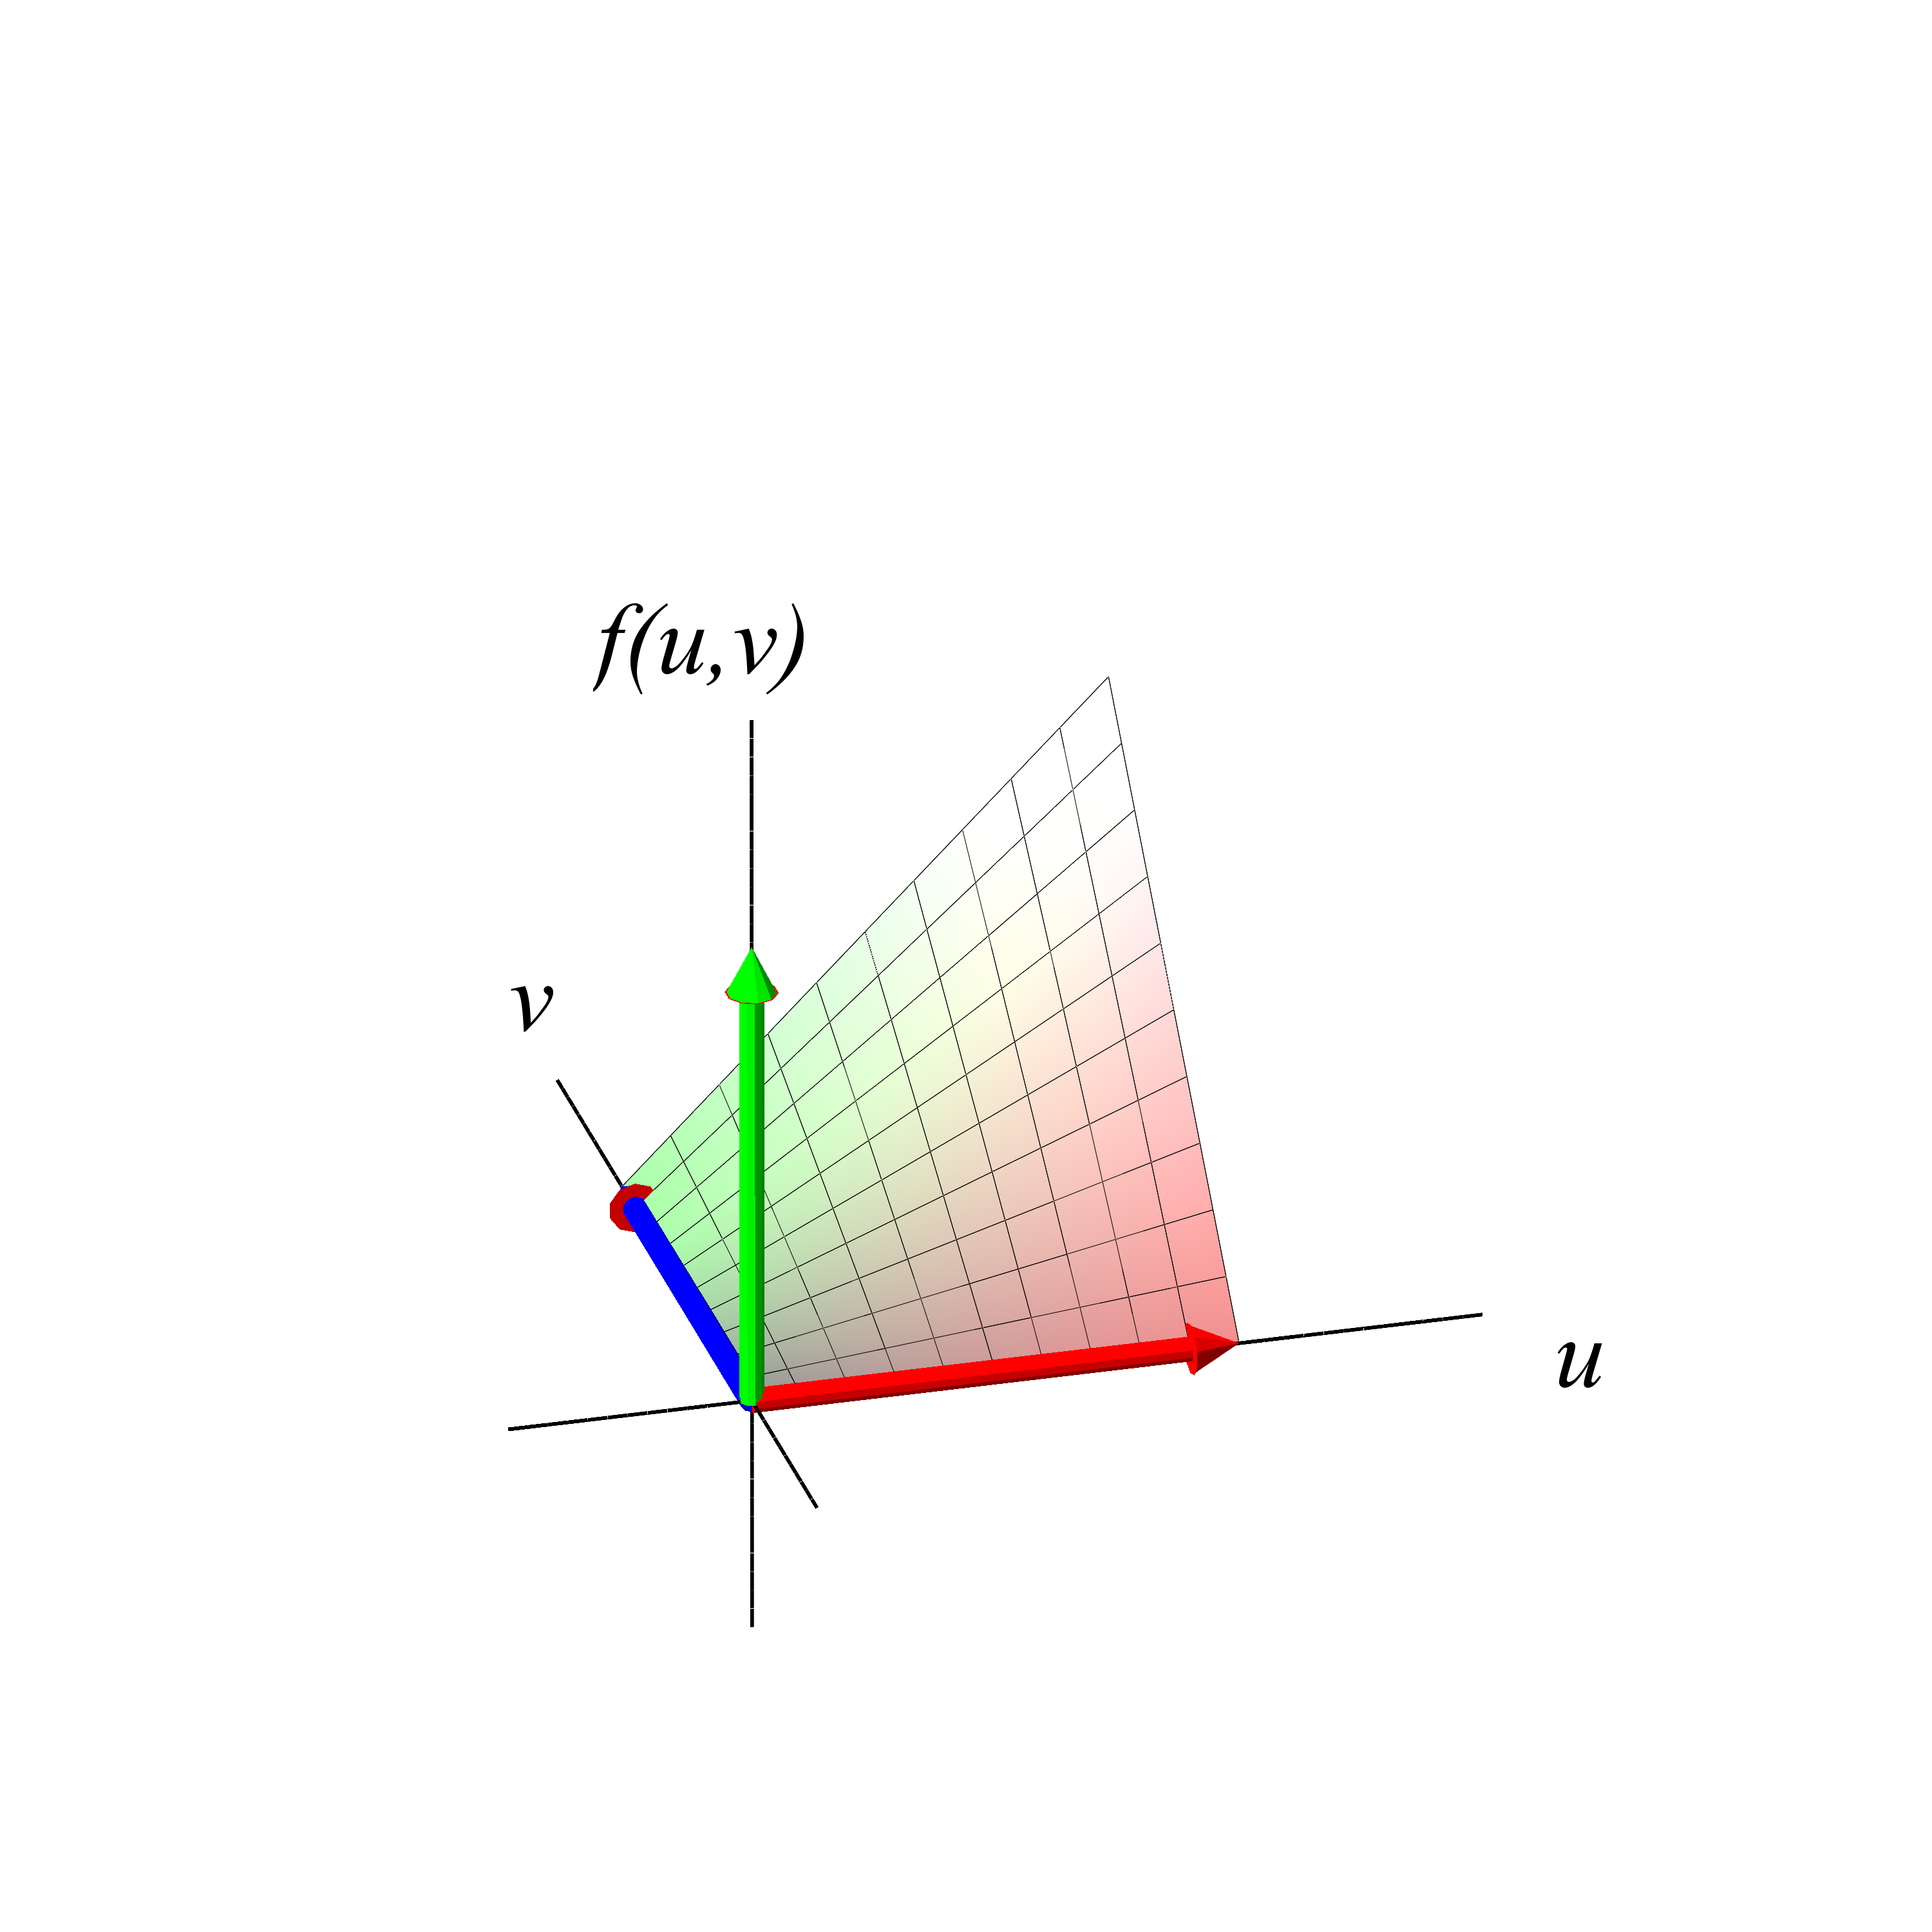
\includegraphics[height=100mm]{FIGS/plotIntuv} \quad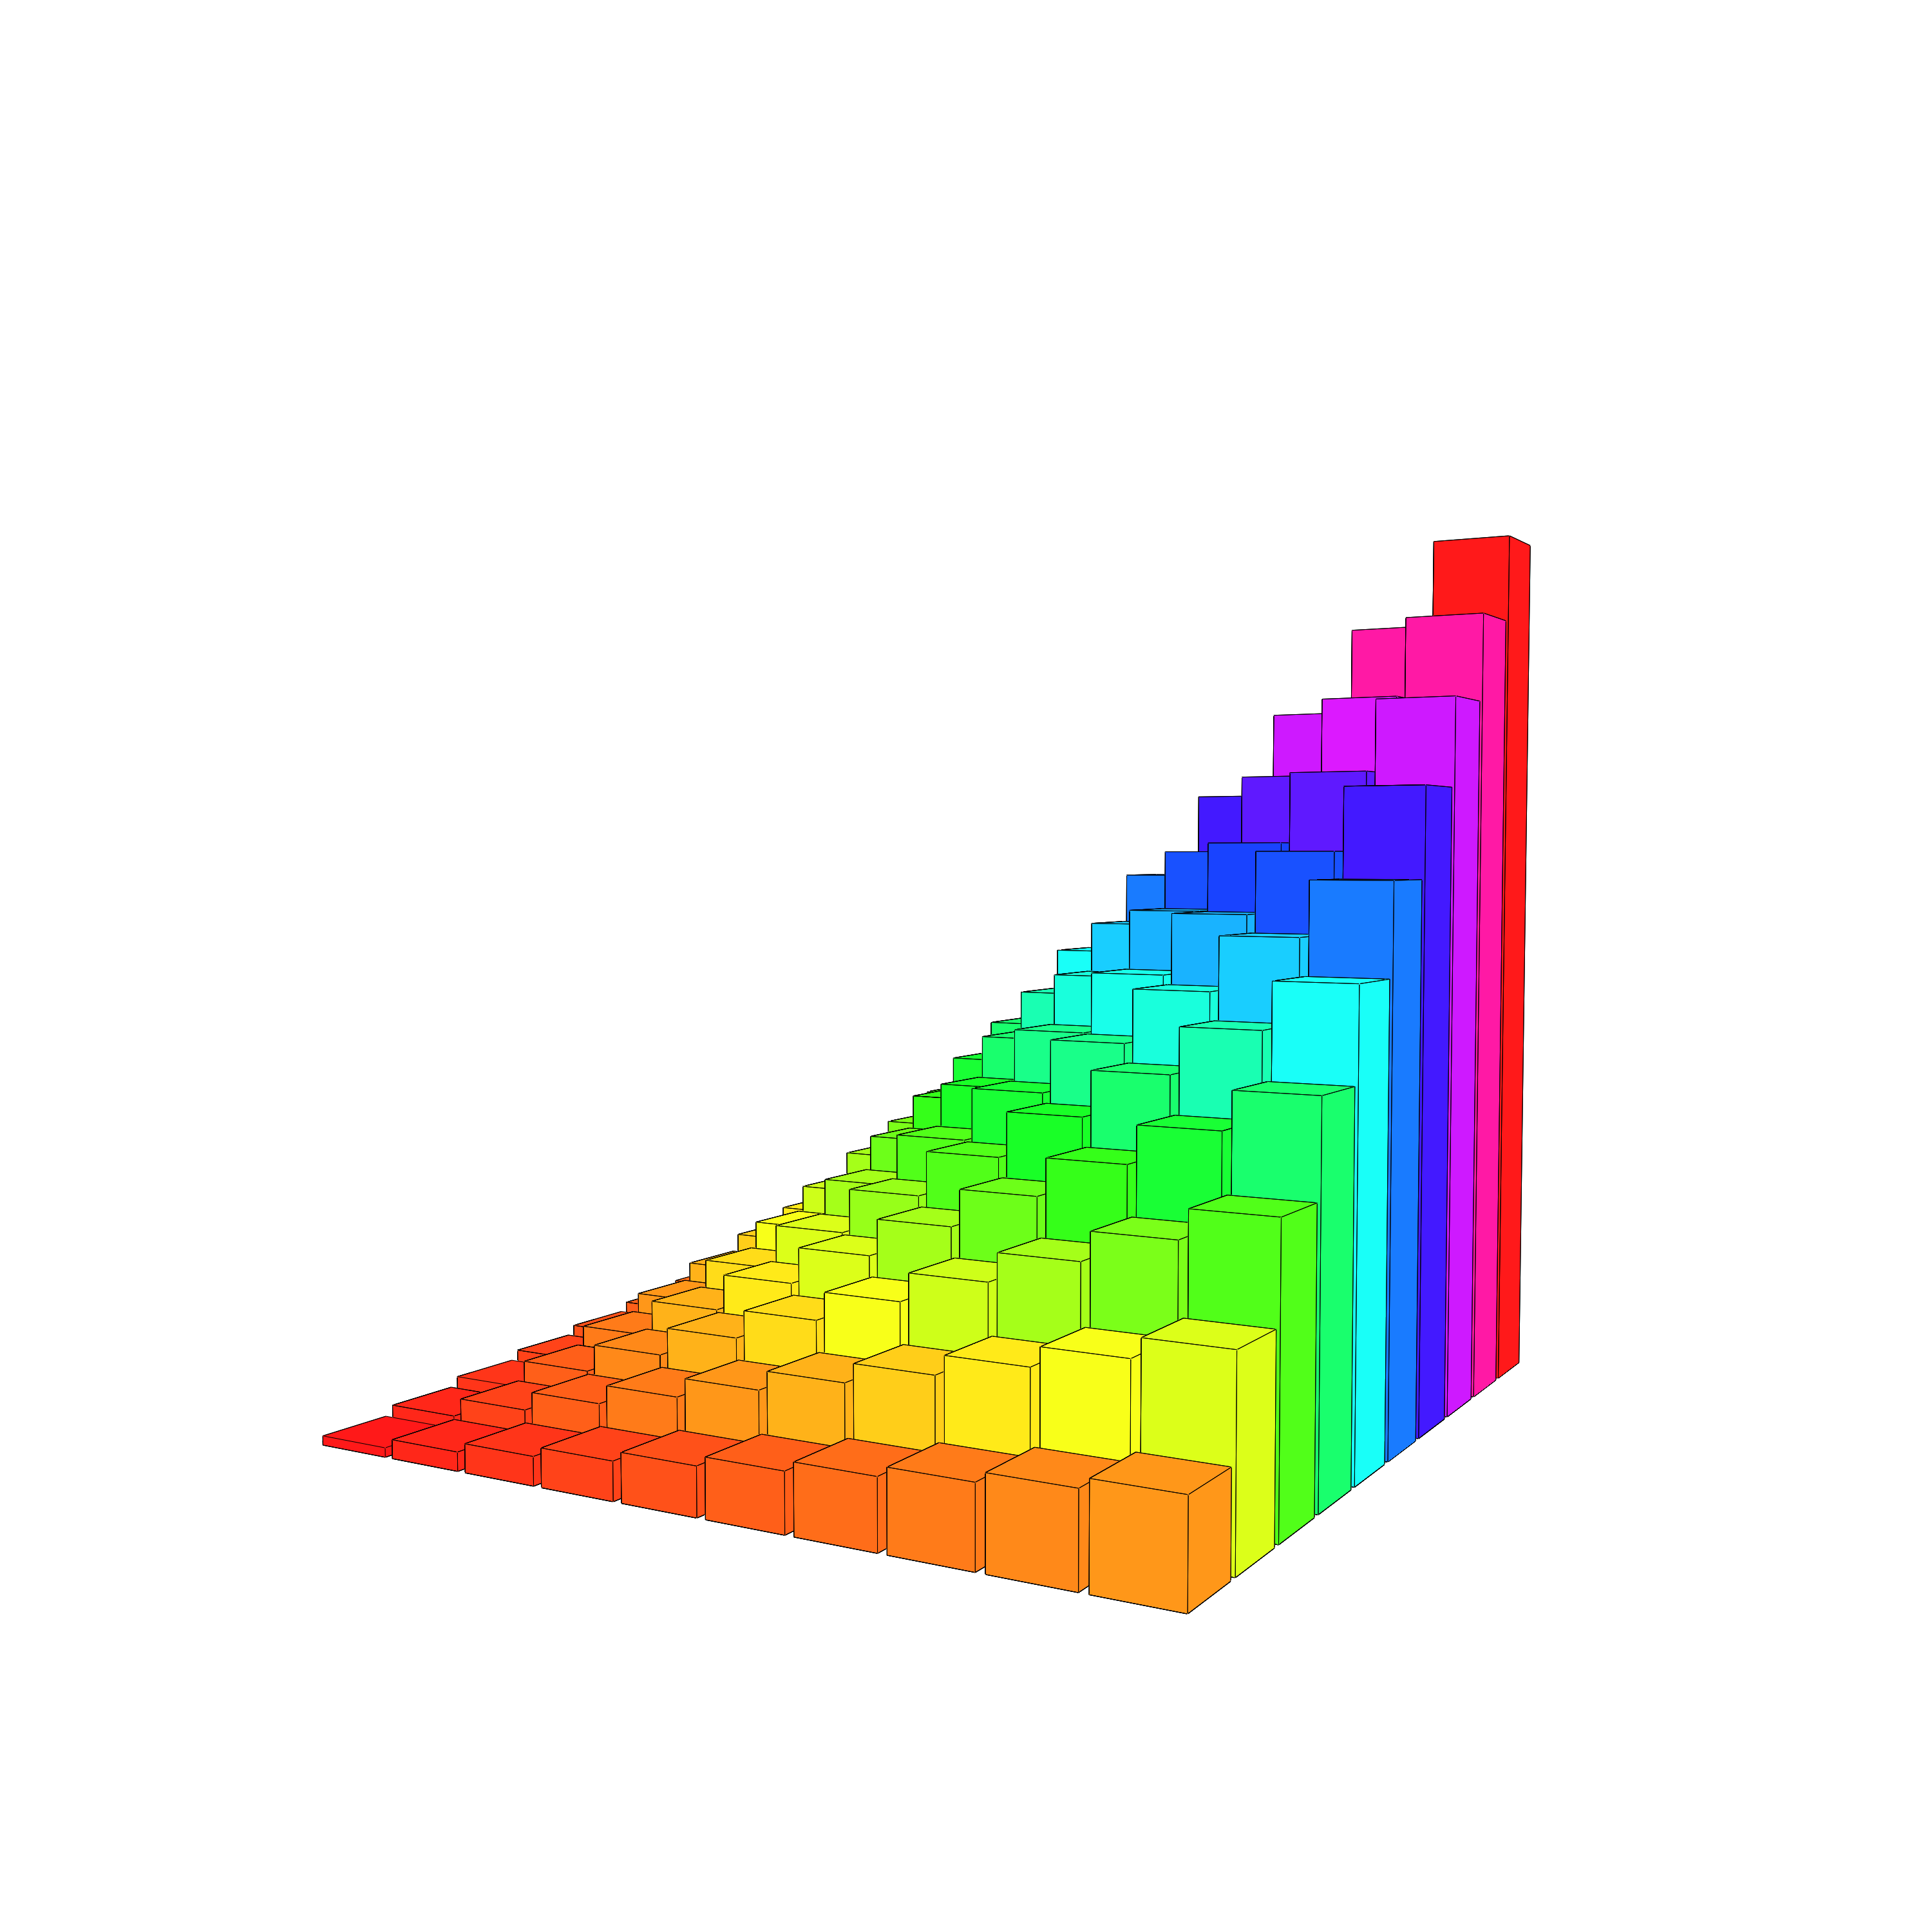
\includegraphics[height=60mm]{FIGS/plotIntuvBox}}
\begin{center}
\caption{\small{Volumen-repræsentation af
integralsummen $\operatorname{II}(f,10, 10, [0,1] \times
[0,1])$  for funktionen $f(u,v) = \,u\,v\,$.}}
\label{FigIIS}
\end{center}
\end{figure}


\begin{example}[Et Riemann'sk dobbeltintegral] \label{exDobbeltInt}
Lad $\,f(u,v) = u \cdot v^{2}\,$ for $\,u \in [\,0,1]\,$ og $\, v \in [-1, 1]\,$. Så er
\begin{equation}
\begin{aligned}
\int_{-1}^{1}\, \left(
\int_{0}^{1} v^{2}\,u du \, \right)\, dv \, &= \, \frac{1}{2}\int_{-1}^{1}\, [\,v^{2}\,u^{2}\,]_{u=0}^{u=1}\, dv \\ &= \,
\frac{1}{2}\int_{-1}^{1}\, v^{2}\, dv \\ &= \,
\frac{1}{6}[\,v^{3}\,]_{v=-1}^{v=1} \\ &= \, \frac{1}{3} \quad .
\end{aligned}
\end{equation}
Bemærk, at beregningen af dobbeltintegralet foretages 'indefra' -- det inderste integral er et integral over $u$-intervallet, her $[0, 1]$, og beregnes først, dvs. med \emph{fastholdt} $v$. En stamfunktion til  $v^{2}\cdot u$ med konstant $v$ er $v^{2} \cdot u^{2}/2$ sådan at:
\begin{equation}
\int_{0}^{1} v^{2}\,cdot u \, du = \frac{1}{2}\cdot[\,v^{2}\,u^{2}\,]_{u=0}^{u=1} = \frac{1}{2}\cdot v^{2} \quad .
\end{equation}
I beregningen kunne vi alternativt have benyttet, at $F_{v}(u) = v^{2}u^{2}/2$ og dermed  $G_{a}(v) = v^{3}a^{2}/6$, $G_{b}(v) = v^{3}b^{2}/6 \,$ og indsat direkte i det sidste udtryk i (\ref{eqDobbeltInt2}).
\end{example}


\begin{example}[Et dobbeltintegral med symmetri] \label{exDobbeltIntUV}
Lad $\,f(u,v) = u\cdot v\,$ for $\,u \in [\,-1,1]\,$ og $\, v \in [-1, 1]\,$. Så er
\begin{equation}
\int_{-1}^{1}\, \left(
\int_{-1}^{1} v\,u \, du \, \right)\, dv \, = \, \frac{1}{2}\int_{-1}^{1}\, [\,v\,u^{2}\,]_{u=-1}^{u=1}\, dv = 0 \quad ,
\end{equation}
mens
\begin{equation}
\begin{aligned}
\int_{0}^{1}\, \left(
\int_{0}^{1} v\,u du \, \right)\, dv \, &= \, \frac{1}{2}\int_{0}^{1}\, [\,v\,u^{2}\,]_{u=0}^{u=1}\, dv  \\
&= \frac{1}{2}\int_{0}^{1}\, v\, dv  \\
&= \frac{1}{2}\cdot \frac{1}{2} \cdot [\,v^{2}\,]_{v=0}^{v=1} \\
&= \frac{1}{4}
\quad .
 \end{aligned}
\end{equation}
\end{example}







\begin{example}[Dobbelt integralsum] \label{exampDobbeltSumUV}
Volumen-repræsentation af
integralsummen $\operatorname{II}(f,10, 10, [0,1] \times
[0,1])$  for funktionen $f(u,v) = \,u\,v\,$ er vist i figur \ref{FigIIS}. De
$100$ addender i summen er til højre repræsenteret ved
søjler med samme kvadratiske tværsnit og med
højder, som er givet ved de respektive værdier af
funktionen $f(u,v) = \,u\,v\,$ i
$(u,v)$-kvadratets delepunkter. Der opnås derved en approksimation til rumfanget
af det område i rummet, der er afgrænset af $(x,y)-$planen og graf-fladen for funktionen
$\,f(x,y) \, = \, xy\,$ over kvadratet $(x, y) \in  [0,1] \times
[0,1]$, som vist til venstre. Det eksakte rumfang er $\frac{1}{4}$.
\end{example}



%%%%%%%%%%%%%%%%%%%%%%%%%%%%%%%%%%%%%%%%%%%%%%
%%%%%%%%%%%%%%%%%%%%%%%%%%%%%%%%%%%%%%%%%%%%%%
%%%%%%%%%%%%%%%%%%%%%%%%%%%%%%%%%%%%%%%%%%%%%%

\section{Tredobbelte summer og tredobbelte integraler} \label{secTreSummer}


\begin{theorem} \label{thmIntIntInt}
Lad $f(u, v, w)$ betegne en kontinuert reel funktion
på et kasseformet parameterområde $[a,b] \times [c,d] \times [h, l]\,$ i $(u,
v, w)$-rummet. Intervallet $[a, b]$ deles i $n$ lige
store delintervaller, intervallet $[c, d]$
deles i $m$ lige store delintervaller, og intervallet $[h, l]$ deles i $q$ lige
store delintervaller. Så har
hvert $u$-delinterval længden $\delta_{u} \, = \,
(b-a)/n$, hvert $v$-delinterval har længden
$\delta_{v} \, = \, (d-c)/m$ og hvert $w$-delinterval har længden
$\delta_{w} \, = \, (h-l)/q$. Tilsvarende bliver
delepunkternes koordinater i $(u,
v, w)$-parameter\-om\-rå\-det
$[a,b]\times[c,d]\times [h, l]$ i $\mathbb{R}^{3}$:

\begin{equation}
\begin{aligned}
(u_{1}, v_{1}, w_{1}) \, &= \, (a, c, h), \\
 &.... \\
(u_{n}, v_{m}, w_{q}) \, &= \, (a + (n-1)\delta_{u}, c + (m-1)\delta_{v}, h + (q-1)\delta_{w})
\quad .
\end{aligned}
\end{equation}
 Lad nu $\,\operatorname{III}(f, n, m, q, [a,b] \times [c,d] \times [h, l])\,$ betegne følgende
 {\emph{\ind{tredobbelte sum}}}:
\begin{equation}\label{eqIIS2}
\begin{aligned}
&\operatorname{III}(f, n, m, q, [a,b] \times [c,d] \times [h, l]) \\ &=
\,\, \sum_{k=1}^{k=q}\,\left( \sum_{j=1}^{j=m}\, \left( \,\sum_{i=1}^{i=n}\, f\left(u_{i}, \,\,\,
v_{j}, \,\,\, w_{k}\,\right)\, \delta_{u} \,\right) \, \delta_{v} \right)\, \delta_{w} \quad .
\end{aligned}
\end{equation}
Så gælder
\begin{equation} \label{eqDobbeltInt3}
\begin{aligned}
&\lim_{n\, \to \infty}\, \left( \,\lim_{m\, \to \infty} \, \left( \,\lim_{q\, \to \infty}\operatorname{III}(f,n,m,q,
[a,b] \times [c,d] \times [h, l])\,\right)\, \right) \\ &= \, \int_{h}^{l}\, \left(\int_{c}^{d}\, \left(
\int_{a}^{b} f(u,v,w)\, du \, \right)\, dv \, \right)\, dw \quad .
\end{aligned}
\end{equation}
\end{theorem}

Summer af typen $\,\operatorname{III}(f,n,m,q,
[a,b] \times [c,d] \times [h, l]\,)\,$ vil vi naturligvis
kalde {\emph{tredobbelte integralsummer}} og grænseværdien $\,\,\int_{h}^{l}\, \left(\int_{c}^{d}\, \left(
\int_{a}^{b} f(u,v,w)\, du \, \right)\, dv \, \right)\, dw\,\,$ kaldes \emph{Riemann-integralet} af $f(u,v,w)$ over $[a, b]\times [c,d] \times [h, l]\,$.



%%%%%%%%%%%%%%%%%%%%%%%%%%%%%%%%%%%%%%%%%%%%%%%%%%%%%%%%%%%%%%%%%%%%%%%%
%%%%%%%%%%%%%%%%%%%%%%%%%%%%%%%%%%%%%%%%%%%%%%%%%%%%%%%%%%%%%%%%%%%%%%%%


\section{Fundamental-sætningen for tredobbelte integralsummer}\label{secFundamIII}

De Riemann'ske tredobbelte integraler beregnes  således:

\begin{theorem}\label{thmAnalyseFundamental3}
Lad $f(u,v,w)$ betegne en kontinuert funktion på $[a, b]\times [c,d] \times [h, l]\,$. \\
Antag, at $F(u,v,w)$ er en (vilkårlig) stamfunktion for $f(u, v, w)$ (betragtet som en funktion af den ene variabel $u$) for vilkårligt givne $v \in [c, d]\,$ og $w \in [h, l]\,$ .
\begin{itemize}
\item Lad $G(a,v,w)$ være en vilkårlig stamfunktion til $F(a, v, w)$ (betragtet som en funktion af den  ene variabel $v$) for vilkårligt givet $w \in [h, l]\,$ .\\
\item Lad $G(b,v,w)$ være en vilkårlig stamfunktion til $F(b, v, w)$ (igen betragtet som en funktion af den  ene variabel $v$) for vilkårligt givet $w \in [h, l]\,$ . \\
\item Lad endelig $H(a, c, w)$ være en vilkårlig stamfunktion til $G(a, c, w)$, og tilsvarende $H(b, c, w)$, $H(a, d, w)$, og $H(b, d, w)$ stamfunktioner for $G(b, c, w)$, $G(a, d, w)$, og $G(b, d, w)\,$.
\end{itemize}
Så gælder :
\begin{equation} \label{eqDobbeltInt3Expand}
\begin{aligned}
&\lim_{n\, \to \infty}\, \left( \,\lim_{m\, \to \infty} \, \left(\,\lim_{q\, \to \infty} \operatorname{III}(f,n,m,q,
[a, b]\times [c,d]\times [h, l])\,\right) \right) \\ &= \,
\int_{h}^{l}\, \left(\int_{c}^{d}\, \left(
\int_{a}^{b} f(u,v,w)\, du \, \right)\, dv \, \right)\, dw \\ &= \,
H(b,d,l)-H(b,d,h) - \left(H(b,c,l) - H(b,c,h)\right) \\
 & \qquad - \left(\left(H(a,d,l)-H(a,d,h)\right) - \left(H(a,c,l)- H(a,c,h)\right)\right)\ \quad .
\end{aligned}
\end{equation}
\end{theorem}
\vspace{0.2cm}


Vi illustrerer med et par simple beregninger:

\begin{example}[Tredobbelt integration] \label{exDobbeltInt3}
Lad $\,f(u,v,w) = u\,v\,\sin(w)\,$ for $\,u \in [\,0,1]\,$,  $\, v \in [\,0, 2]\,$ og $\, w \in [\,0, \pi/2]\,$. Så er
\begin{equation*}
\begin{aligned}
\int_{0}^{\pi/2}\left(\int_{0}^{2}\, \left(
\int_{0}^{1} u\,v \, \sin(w)\, du \, \right)\, dv\, \right)\, dw \, &= \,
\int_{0}^{\pi/2}\left(\int_{0}^{2}\,
 v \, \sin(w) \,[\,u^{2}/2\,]_{u=0}^{u=1}\,\, dv\, \right)\, dw \\ &= \,
\frac{1}{2}\int_{0}^{\pi/2}\left(\int_{0}^{2}\,
 v \, \sin(w)\, dv\, \right)\, dw \\ &= \,
\frac{1}{2}\int_{0}^{\pi/2}
\sin(w)\,[\,v^{2}/2 \,]_{v=0}^{v=2}\,\, dw \\ &= \,
\int_{0}^{\pi/2}
\sin(w)\, dw \\ &= \,
[-\cos(w)]_{w=0}^{w=\pi/2} \\ &= \,
1 \quad .
\end{aligned}
\end{equation*}
\end{example}



\begin{example}[Et tre-dobbeltintegral med symmetri] \label{exampTreDobbeltIntUVW}
Lad $\,f(u,v,w) = u\cdot v\cdot w \,$ for $\,u \in [\,-1,1]\,$ og $\, v \in [-1, 1]\,$, og $\, w \in [-1, 1]\,$. Så er
\begin{equation}
\int_{-1}^{1}\, \left(\int_{-1}^{1}\, \left(
\int_{-1}^{1} w\,v\,u \, du \, \right)\, dv \, \right) \, dw =  0 \quad ,
\end{equation}
mens
\begin{equation}
\int_{0}^{1}\, \left(\int_{0}^{1}\, \left(
\int_{0}^{1} w\,v\,u \, du \, \right)\, dv \, \right) \, dw =  \frac{1}{8} \quad ,
\end{equation}
\end{example}





\begin{example}[Enhedskuglens rumfang] \label{exampKugle}
Som gennemgået i eNoten om integration over rumlige områder beregnes volumenet af den massive enhedskugle ved følgende tredobbelte Riemann-integral (som vil blive motiveret i den eNote). Dermed verificeres {Archimedes'
resultat}:
\begin{equation}
\begin{aligned}
\Vol(\rm{Enhedskuglen}) \, &= \, \int_{0}^{1}\left(\int_{-\pi}^{\pi}\, \left(
\int_{0}^{\pi} w^{2}\sin(u)\, du \, \right)\, dv\, \right)\, dw  \\
&= \,
\int_{0}^{1}\left(\int_{-\pi}^{\pi}\,
w^{2} \,[\,-\cos(u)\,]_{u=0}^{u=\pi}\,\,\, dv\, \right)\, dw \\ &= \,
2\int_{0}^{1}\left(\int_{-\pi}^{\pi}\,
 w^{2}\, dv\, \right)\, dw \\ &= \,
2\int_{0}^{1}
w^{2}\,[\,v \,]_{v=-\pi}^{v=\pi}\,\,\, dw \\ &= \,
4\pi \int_{0}^{1}
w^{2}\, dw \\ &= \,
4\pi\,[w^{3}/3\,]_{w=0}^{w=1} \\ &= \,
\frac{4\pi}{3} \quad .
\end{aligned}
\end{equation}
\end{example}




%%%%%%%%%%%%%%%%%%%%%%%%%%%%%%%%%%%%%%%%%%%%%%%%%%%
%%%%%%%%%%%%%%%%%%%%%%%%%%%%%%%%%%%%%%%%%%%%%%%%%%%
%%%%%%%%%%%%%%%%%%%%%%%%%%%%%%%%%%%%%%%%%%%%%%%%%%%
%%%%%%%%%%%%%%%%%%%%%%%%%%%%%%%%%%%%%%%%%%%%%%%%%%%












%%%%%%%%%%%%%%%%%%%%%%%%%%%%%%%%%%%%%%%%%%%%%%%%%%%%%%%%%%%%%
%%%%%%%%%%%%%%%%%%%%%%%%%%%%%%%%%%%%%%%%%%%%%%%%%%%%%%%%%%%%%
%%%%%%%%%%%%%%%%%%%%%%%%%%%%%%%%%%%%%%%%%%%%%%%%%%%%%%%%%%%%%

\begin{summary}
I denne eNote har vi beskæftiget os med basis for de metoder og resultater, der er helt uomgåelige hjælpemidler for at kunne finde
længder, arealer, rumfang, massemidtpunkter, inertimomenter etc. af henholdsvis kurver, og områder i plan og rum.\\
\begin{itemize}

\item For enhver  given kontinuert funktion $f(u)$ af \'{e}n variabel $u$ på et interval $[a, b]$ opstiller vi de integralsummer $\operatorname{I}(f,n, [a, b])$, der i grænsen for $n\to \infty$
definerer  Riemann-integralet af funktionen over intervallet.  Disse Riemann-integraler kan derefter selv beregnes (via fundamentalsætningen)  ved hjælp af en stamfunktion $F(u)$ for $f(u)$ således:
\begin{equation}
\begin{aligned}
\operatorname{I}(f,n, [a, b]) &=  \sum_{i=1}^{i=n}\, f\left(u_{i}\right)\,\delta_{u} \\
 \sum_{i=1}^{i=n}\, f\left(u_{i}\right)\,\delta_{u}  &\to \int_{a}^{b} f(u)\, du \quad \rm{for}\quad  n \to \infty \\
\int_{a}^{b} f(u)\, du  &= \left[F(u)\right]_{u=a}^{u=b} \, \,  = F(b) - F(a) \quad ,
\end{aligned}
\end{equation}
hvor
\begin{equation}
u_{i}= a + (i-1)\cdot \delta_{u} \quad \textrm{og} \quad \delta_{u} = \frac{b-a)}{n} \quad .
\end{equation}
\item Helt tilsvarende grænseværdier for tilsvarende summer for kontinuerte funktioner af to og tre variable er opstillet og eksemplificeret.
\end{itemize}
\end{summary}


%%%%%%%%%%%%%%%%%%%%%%%%%%%%%%%%%%%%%%%%%%%%%
%%%%%%%%%%%%%%%%%%%%%%%%%%%%%%%%%%%%%%%%%%%%%
%%% HER SKAL DU STOPPE MED AT SKRIVE %%%%%%%%
%%%%%%%%%%%%%%%%%%%%%%%%%%%%%%%%%%%%%%%%%%%%%
%%%%%%%%%%%%%%%%%%%%%%%%%%%%%%%%%%%%%%%%%%%%%


\end{document} 

%%%%%%%%%%%%%%%%%%%%%%%%%%%%%%%%%%%%%%%%%%%%%%%%%%%
%%%%%%%%%%%%%%%%%%%%%%%%%%%%%%%%%%%%%%%%%%%%%%%%%%%

